\chapter{Triển khai bằng PyTorch và đánh giá số}
\label{chap:thucnghiem}
 
Chương~\ref{chap:pinn} đã thiết lập bằng chứng minh một loạt phát biểu về hành vi
của mạng nơ-ron thông tin vật lý: điều kiện chính quy bắt buộc lên hàm kích hoạt,
chặn ổn định nối phần dư với sai số, cơ chế khuếch đại phổ của toán tử vi phân, và
tính không khả thi của việc học trọng số cân bằng bằng hạ gradient. Mọi phát biểu
ấy đều là những khẳng định \emph{kiểm chứng được}. Chương này thực hiện việc kiểm
chứng đó.
 
Mục tiêu không dừng ở chỗ trình bày một cài đặt chạy được. Mỗi thí nghiệm dưới
đây được thiết kế để trả lời một câu hỏi cụ thể do Chương~\ref{chap:pinn} đặt ra,
với tiêu chí thành công hoặc thất bại xác định \emph{trước} khi chạy. Ta báo cáo
đầy đủ cả những chỗ khớp lẫn những chỗ không khớp: trong mười bốn hạng mục đối
chiếu ở Mục~\ref{sec:doi-chieu}, sáu khớp trọn vẹn, hai khớp về hướng nhưng
không về độ lớn, \emph{bốn} buộc phải siết lại cách phát biểu, một không tái lập
được khi đổi hạt giống, và một cho kết quả trái với kỳ vọng.
Phần điều chỉnh được ghi rõ thay vì bỏ qua; theo quan điểm của báo cáo, một kết
quả tiêu cực được phân tích đúng nguyên nhân có giá trị ngang một kết quả khớp.
 
Cấu trúc chương: Mục~\ref{sec:trienkhai} mô tả kiến trúc cài đặt trên
PyTorch~\cite{paszke2019} và cấu hình chung. Các
Mục~\ref{sec:tn1}--\ref{sec:tn10} trình bày mười thí nghiệm.
Mục~\ref{sec:doi-chieu} đối chiếu toàn bộ lý thuyết với số liệu, và
Mục~\ref{sec:hanche} nêu thẳng những hạn chế của thiết kế thực nghiệm này.
 
%==============================================================================
\section{Kiến trúc triển khai}
\label{sec:trienkhai}
%==============================================================================
 
\subsection{Đồ thị tính toán động và vi phân tự động lồng nhau}
\label{ssec:ad-pytorch}
 
Đặc điểm khiến PyTorch phù hợp với PINNs là cơ chế \emph{đồ thị tính toán động}
(define-by-run): đồ thị theo Định nghĩa~\ref{def:comp-graph} được dựng lại ở mỗi
lượt xuôi, do đó bản thân \emph{đạo hàm} cũng là một đỉnh trong đồ thị và có thể
tiếp tục vi phân được~\cite{paszke2019}.
 
Theo Mệnh đề~\ref{md:ad-tai-tao}, việc tính $\nabla_{\btheta}r_{\btheta}$ đòi hỏi
vi phân một biểu thức vốn đã chứa $\partial_{\bxi}u_{\btheta}$. Điều kiện kỹ thuật
để thực hiện được là truyền cờ \texttt{create\_graph=True} vào
\texttt{torch.autograd.grad}: cờ này yêu cầu giữ lại đồ thị của phép tính đạo hàm
thay vì giải phóng nó. Nếu thiếu cờ, lời gọi \texttt{backward()} tiếp theo sẽ báo
lỗi hoặc -- nguy hiểm hơn -- trả về gradient bằng không mà không cảnh báo, đúng
tình huống đã nêu ở cuối Mục~\ref{subsec:bac-cao-ad}.
 
\begin{lstlisting}[caption={Toán tử đạo hàm lồng nhau theo biến đầu vào.},label={lst:grad}]
def grad(y, x, order=1):
    """Dao ham cap `order` cua y theo x, giu lai do thi de vi phan tiep."""
    for _ in range(order):
        y = torch.autograd.grad(y, x, torch.ones_like(y),
                                create_graph=True)[0]
    return y
\end{lstlisting}
 
Hàm ở Đoạn mã~\ref{lst:grad} là hiện thực trực tiếp của các công thức truy hồi
\eqref{eq:G-truy-hoi} và \eqref{eq:S-truy-hoi}: mỗi lần lặp trong vòng
\texttt{for} tương ứng với một bậc trong truy hồi Jacobi--Hessian
(Mệnh đề~\ref{md:jacobian} và \ref{md:hessian}), và chi phí nhân lên theo hệ số
hằng đúng như Nhận xét~\ref{nx:chi-phi-bac-cao} dự báo. Cần lưu ý rằng vectơ
$\texttt{torch.ones\_like(y)}$ ở đối số thứ ba chính là vectơ mầm $\bm{w}$ trong
định nghĩa biến liên hợp \eqref{eq:adjoint}: hàm này thực hiện một tích
vectơ--Jacobi \eqref{eq:vjp}, không dựng ma trận Jacobi.

\begin{nhanxet}[Vì sao viết lại thay vì dùng thư viện đóng gói]
\label{nx:vi-sao-tu-viet}
Đã có thư viện PINNs trưởng thành, tiêu biểu là DeepXDE của Lu và cộng
sự~\cite{lu2021}. Phần~2 của bài báo ấy mô tả một thiết kế tách bài toán thành
các thành phần độc lập --- hình học miền, đối tượng điều kiện biên, đối tượng dữ
liệu, và một lớp mô hình lo phần huấn luyện --- rồi ghép chúng lại. Cách tổ chức ấy là đúng cho \emph{người dùng}
phương pháp: nó giấu đi đúng những chi tiết mà báo cáo này lấy làm đối tượng
khảo sát.

Ba thí nghiệm của chương này chỉ đặt ra được khi ta cầm trực tiếp các chi tiết
đó. Thí nghiệm~\ref{tn:relu} cần đọc $\nabla_{\btheta}J_r$ \emph{trước} khi bộ
tối ưu chạm vào nó, để thấy nó bằng đúng không. Mục~\ref{sec:tn4} và~\ref{sec:tn5} cần tách
riêng gradient của từng thành phần mất mát ở mỗi vòng lặp --- một phép đo không
nằm trong giao diện huấn luyện thông thường. Và cùng hai mục ấy cần
can thiệp vào chính quy tắc cập nhật $\lambda_i$ để quan sát chế độ phản hồi
dương của Bổ đề~\ref{bd:phan-hoi-duong}. Nói ngắn gọn: thư viện tối ưu hoá cho
việc \emph{giải} phương trình, còn báo cáo này cần quan sát \emph{cơ chế} của
bộ giải.

Điều đi vay từ~\cite{lu2021} là các quy ước đo và đối chiếu, chứ không phải mã
nguồn: dùng sai số $L^2$ tương đối làm chỉ tiêu chính, đối chiếu thẳng với một
bộ giải cổ điển trên cùng bài toán (Mục~\ref{sec:tn9}), và lấy phần dư làm tín
hiệu chẩn đoán --- ý tưởng đứng sau lấy mẫu thích nghi RAR ở
Bảng~\ref{tab:remedies}, mà Mục~\ref{sec:hanche} ghi nhận là hướng đáng thử
trước tiên cho bài toán Burgers.
\end{nhanxet}
 
\subsection{Mạng nơ-ron và khởi tạo}
 
\begin{lstlisting}[caption={Mạng truyền thẳng với khởi tạo Xavier và nhúng đặc trưng Fourier tuỳ chọn.},label={lst:fnn}]
class FNN(nn.Module):
    def __init__(self, layers, act="tanh", fourier_m=0, fourier_s=1.0):
        super().__init__()
        self.fourier_m = fourier_m
        if fourier_m > 0:                      # nhung dac trung Fourier
            B = torch.randn(fourier_m, layers[0]) * fourier_s
            self.register_buffer("B", B)       # B co dinh, khong hoc
            layers = [2 * fourier_m] + layers[1:]
        self.lins = nn.ModuleList(
            [nn.Linear(layers[i], layers[i+1]) for i in range(len(layers)-1)])
        for lin in self.lins:                  # khoi tao Xavier (Muc 2.3)
            nn.init.xavier_normal_(lin.weight)
            nn.init.zeros_(lin.bias)
        self.act = {"tanh": torch.tanh, "relu": torch.relu}[act]
 
    def forward(self, x):
        if self.fourier_m > 0:
            p = 2 * math.pi * x @ self.B.T
            x = torch.cat([torch.cos(p), torch.sin(p)], dim=1)
        for lin in self.lins[:-1]:
            x = self.act(lin(x))
        return self.lins[-1](x)
\end{lstlisting}
 
Ba lựa chọn trong Đoạn mã~\ref{lst:fnn} tương ứng trực tiếp với ba kết luận của
Chương~\ref{chap:fnn}. Khởi tạo Xavier là \eqref{eq:xavier} với độ chệch bằng
$\bm{0}$, đúng quy ước (A2) của Mục~\ref{subsec:phuong-sai}; ta dùng dạng
\emph{chuẩn tắc} (\texttt{xavier\_normal\_}) chứ không phải dạng đều
\eqref{eq:xavier-uniform}, và theo Nhận xét~\ref{nx:xavier-dang} hai dạng cho
cùng phương sai nên mọi kết quả của Chương~\ref{chap:fnn} áp dụng như nhau. Vòng lặp
\texttt{for lin in self.lins[:-1]} bỏ hàm kích hoạt ở lớp cuối, hiện thực quy ước
lớp ra tuyến tính \eqref{eq:fnn-output}. Ma trận $B$ của nhúng Fourier được đăng
ký bằng \texttt{register\_buffer} chứ không phải \texttt{Parameter}: nó cố định,
không tham gia tối ưu -- một quyết định thiết kế sẽ được kiểm chứng ở
Thí nghiệm~\ref{tn:pho}.
 
Toàn bộ tính toán dùng \texttt{float64}. Lựa chọn này không tuỳ tiện. Ở giai đoạn
L-BFGS, $J_r$ cần đạt tới bậc $10^{-8}$ hoặc nhỏ hơn, trong khi \texttt{float32}
chỉ có khoảng bảy chữ số thập phân có nghĩa. Quan trọng hơn, theo
Nhận xét~\ref{nx:fd-pde}, sai số ở phần dư không bị dập tắt mà được khuếch đại
qua toàn bộ quá trình huấn luyện; độ chính xác kép là điều kiện cần để phân biệt
sai số xấp xỉ với sai số làm tròn, tức để các con số trong chương này có nghĩa.
 
\subsection{Phần dư và quy trình huấn luyện hai giai đoạn}
 
\begin{lstlisting}[caption={Phần dư của phương trình Burgers và vòng huấn luyện.},label={lst:train}]
def residual(net, X):                 # X = (x, t), yeu cau requires_grad_(True)
    u  = net(X)
    g  = grad(u, X)                   # [du/dx, du/dt]
    ut, ux = g[:, 1:2], g[:, 0:1]
    uxx = grad(ux, X)[:, 0:1]         # dao ham bac hai -> can create_graph
    return ut + u * ux - NU * uxx
 
# --- Giai doan 1: Adam ---
opt = torch.optim.Adam(net.parameters(), lr=1e-3)
for it in range(adam_iters + 1):
    Jr = (residual(net, Xr) ** 2).mean()
    Jb = (net(Xb) ** 2).mean()        # hop le vi g == 0 tren bien
    J0 = ((net(X0) - u0) ** 2).mean()
    J  = Jr + lam_b * Jb + lam_0 * J0
    opt.zero_grad(); J.backward(); opt.step()
 
# --- Giai doan 2: L-BFGS voi tim kiem duong Wolfe manh ---
opt2 = torch.optim.LBFGS(net.parameters(), max_iter=800, history_size=50,
                         line_search_fn="strong_wolfe")
opt2.step(closure)
\end{lstlisting}
 
Quy trình hai giai đoạn ở Đoạn mã~\ref{lst:train} hiện thực đúng
Thuật toán~\ref{alg:two-stage}, được lập luận ở Mục~\ref{subsec:adam-vs-lbfgs}
bằng ba lý do: tính tất định của gradient, sàn nhiễu
(Mệnh đề~\ref{md:san-nhieu}), và điều kiện xấu. Tham số
\texttt{line\_search\_fn="strong\_wolfe"} không phải tuỳ chọn: theo
Bổ đề~\ref{bd:wolfe-curvature}, nó là điều kiện để $\bm{H}_k$ giữ tính xác định
dương. Hiệu quả định lượng của bước chuyển được đo ở Mục~\ref{sec:tn4}.
 
Một chi tiết cài đặt đáng nêu: dòng \texttt{Jb = (net(Xb) ** 2).mean()} chỉ đúng
vì mọi bài toán trong chương có điều kiện biên thuần nhất $g \equiv 0$. Với
$g \not\equiv 0$ phải viết \texttt{((net(Xb) - g\_b) ** 2).mean()}. Ta nêu vì đây
là lỗi im lặng: chương trình vẫn chạy và hàm mục tiêu vẫn giảm.
 
\subsection{Công cụ đo: chỉ số mất cân bằng gradient}
\label{ssec:rho}
 
Để đo bệnh lý gradient ở Mục~\ref{sec:gradient-pathology} một cách định lượng, ta
dùng chính đại lượng xuất hiện trong quy tắc \eqref{eq:lambda-hat} của
Thuật toán~\ref{alg:annealing}.
 
\begin{definition}[Chỉ số mất cân bằng gradient]
\label{dn:rho}
Với hàm mục tiêu ở dạng \eqref{eq:loss-compact}, \emph{chỉ số mất cân bằng} của
thành phần thứ $i$ tại tham số $\btheta$ là
\begin{equation}
\rho_i(\btheta)
 := \frac{\norm{\nabla_{\btheta} J_r(\btheta)}_{\infty}}
         {\tfrac{1}{P}\norm{\nabla_{\btheta} J_i(\btheta)}_{1}} .
\label{eq:rho}
\end{equation}
Ta nói bài toán \emph{mắc bệnh lý gradient} đối với thành phần $i$ nếu
$\rho_i \gg 1$ \emph{và} $\rho_i$ tăng theo số vòng lặp huấn luyện.
\end{definition}
 
Điều kiện thứ hai trong Định nghĩa~\ref{dn:rho} là điều kiện thực chất và cần
được nhấn mạnh, vì bài toán khuếch tán ở Mục~\ref{sec:tn4} sẽ cho thấy một
bài toán có
$\rho_b = 25{,}4$ tại khởi tạo nhưng \emph{giảm} sau đó, và việc can thiệp vào bài
toán ấy phản tác dụng. Giá trị tuyệt đối của $\rho_i$ tại một thời điểm không đủ
để chẩn đoán; xu hướng mới đủ.
 
\begin{lstlisting}[caption={Đo chỉ số mất cân bằng $\rho_i$ theo \eqref{eq:rho}.},label={lst:rho}]
def imbalance(loss_r, loss_i, params):
    """rho_i = max|grad J_r| / mean|grad J_i|   (Dinh nghia 5.1)."""
    gr = flat_grad(loss_r, params)     # can retain_graph=True
    gi = flat_grad(loss_i, params)
    return gr.abs().max().item() / gi.abs().mean().item()
\end{lstlisting}
 
Theo Mệnh đề~\ref{md:chi-phi-bp}, mỗi lượt ngược riêng rẽ tốn xấp xỉ chi phí một
lượt xuôi, nên việc đo $\rho_i$ đắt gấp $M+1$ lần một bước huấn luyện thường. Ta
chỉ đo mỗi $100$ vòng lặp.
 
\subsection{Cấu hình thí nghiệm và chỉ tiêu đánh giá}
\label{ssec:cauhinh}
 
\begin{table}[H]
\centering
\caption{Cấu hình chung của các thí nghiệm. Mọi lần chạy dùng hạt giống cố định
để tái lập được; hạn chế của lựa chọn này được nêu ở Mục~\ref{sec:hanche}.}
\label{tab:cauhinh}
\small
\begin{tabular}{@{}p{4.3cm}p{9.2cm}@{}}
\toprule
\textbf{Hạng mục} & \textbf{Thiết lập} \\
\midrule
Thư viện & PyTorch, NumPy; độ chính xác \texttt{float64} \\
Phần cứng & 1 lõi CPU, không dùng GPU \\
Hàm kích hoạt & $\tanh$ (trừ thí nghiệm đối chứng ReLU ở Mục~\ref{sec:tn1}) \\
Khởi tạo & Xavier dạng chuẩn tắc, $\Var(w^{(\ell)}) = 2/(n_{\ell-1}+n_{\ell})$
  theo \eqref{eq:xavier}; $\bb^{(\ell)} = \bm{0}$ \\
Kiến trúc bài toán 1D & $(1,32,32,32,1)$, $2\,209$ tham số \\
Kiến trúc bài toán 2D & $(2,32,32,32,32,1)$, $3\,297$ tham số \\
Kiến trúc bài toán đa tần số & $(1,64,64,64,1)$, $8\,513$ tham số \\
Tối ưu giai đoạn 1 & Adam, $\eta = 10^{-3}$, $\beta = (0{,}9;\,0{,}999)$ \\
Tối ưu giai đoạn 2 & L-BFGS, \texttt{history\_size}${}=50$, Wolfe mạnh \\
Lấy mẫu điểm phối trí & Lưới đều (1D) hoặc lấy mẫu đều ngẫu nhiên (2D) \\
\bottomrule
\end{tabular}
\end{table}
 
Số tham số trong Bảng~\ref{tab:cauhinh} khớp với công thức \eqref{eq:so-tham-so}:
với kiến trúc $(1,32,32,32,1)$ ta có
$P = (1\cdot32+32) + 2\times(32\cdot32+32) + (32\cdot1+1) = 64 + 2112 + 33
= 2\,209$.
 
\begin{definition}[Chỉ tiêu sai số]
\label{dn:chi-tieu}
Gọi $\{\bxi_j\}_{j=1}^{M}$ là lưới đánh giá, \emph{khác} với tập điểm phối trí
huấn luyện, và $u^{\star}$ là nghiệm đúng hoặc nghiệm tham chiếu. Ta dùng
\begin{equation}
\varepsilon_{L^2}
 := \frac{\Big(\sum_{j}\abs{u_{\btheta}(\bxi_j)
      - u^{\star}(\bxi_j)}^2\Big)^{1/2}}
         {\Big(\sum_{j}\abs{u^{\star}(\bxi_j)}^2\Big)^{1/2}},
\qquad
\varepsilon_{L^{\infty}}
 := \max_{j}\abs{u_{\btheta}(\bxi_j) - u^{\star}(\bxi_j)}.
\label{eq:chi-tieu}
\end{equation}
\end{definition}
 
Việc đánh giá trên lưới \emph{khác} tập huấn luyện là bắt buộc chứ không phải cẩn
trọng thừa. Nhận xét~\ref{rem:monte-carlo} đã lập luận rằng $J_r$ mất tính không
chệch ngay khi $\btheta$ được tối ưu trên chính tập mẫu sinh ra nó: giá trị $J_r$
cuối cùng là ước lượng chệch xuống của $\norm{r_{\btheta}}^2_{L^2}$. Sai số đo
trên lưới độc lập mới phản ánh chất lượng nội suy thực sự.
 
%==============================================================================
\section{Thí nghiệm 1: hàm kích hoạt và sự suy biến của ReLU}
\label{sec:tn1}
%==============================================================================
 
\begin{thinghiem}[Kiểm chứng Hệ quả~\ref{hq:pinn-hong}]
\label{tn:relu}
Hệ quả~\ref{hq:pinn-hong} khẳng định mạng ReLU cho
$\partial_{xx}u_{\btheta} = 0$ hầu khắp nơi
(Hệ quả~\ref{hq:relu-hkn}), dẫn tới $J_r$ hằng địa phương với giá trị
$\overline{f^2}$ và $\nabla_{\btheta}J_r \equiv \bm{0}$. Đây là khẳng định về
\emph{đẳng thức chính xác}, không phải về ``hội tụ chậm'', nên có thể kiểm chứng
tới từng chữ số máy.
\end{thinghiem}
 
\textbf{Thiết lập.} Bài toán Poisson một chiều với nghiệm chế tạo:
\begin{equation}
-u''(x) = f(x) \ \text{ trên } (0,1),
\qquad u(0) = u(1) = 0,
\qquad u^{\star}(x) = \sin(2\pi x),
\label{eq:poisson-tn1}
\end{equation}
do đó $f(x) = 4\pi^2\sin(2\pi x)$. Đây chính là bài toán của
Mệnh đề~\ref{md:chan-on-dinh}, nên ta có sẵn chặn ổn định
$\norm{e_{\btheta}}_{L^2} \le \pi^{-2}\norm{r_{\btheta}}_{L^2}$ để đối chiếu.
Huấn luyện $4\,000$ vòng Adam với $256$ điểm phối trí đều, $\lambda_b = 100$, hai
hàm kích hoạt $\tanh$ và ReLU trên cùng kiến trúc và cùng hạt giống.
 
\begin{table}[H]
\centering
\caption{So sánh hai hàm kích hoạt trên bài toán Poisson \eqref{eq:poisson-tn1}.}
\label{tab:tn1}
\small
\begin{tabular}{@{}lrrrr@{}}
\toprule
\textbf{Hàm kích hoạt} & $\varepsilon_{L^2}$ & $\varepsilon_{L^{\infty}}$
& $J_r$ cuối & $\norm{\nabla_{\btheta}J_r}_{\infty}$ \\
\midrule
$\tanh$ & $5{,}977\times10^{-5}$ & $8{,}701\times10^{-5}$
        & $2{,}463\times10^{-3}$ & --- \\
ReLU    & $9{,}991\times10^{-1}$ & $1{,}004\times10^{0}$
        & $7{,}762\times10^{2}$  & $0{,}0$ \\
\bottomrule
\end{tabular}
\end{table}
 
\textbf{Kết quả.} Ba con số dưới đây là bằng chứng trực tiếp cho từng khẳng định
của Hệ quả~\ref{hq:pinn-hong}.
 
\begin{enumerate}[label=(\alph*),leftmargin=2.2em,itemsep=3pt]
\item \emph{Đạo hàm bậc hai triệt tiêu.} Đo trực tiếp trên mạng ReLU tại khởi tạo
cho $\max_{x}\abs{\partial_{xx}u_{\btheta}(x)} = 0{,}0$ \emph{chính xác} -- không
phải một số nhỏ -- vì \texttt{autograd} truyền $\sigma'' \equiv 0$ qua toàn bộ đồ
thị, đúng theo truy hồi \eqref{eq:ad-hvp}: số hạng thứ nhất triệt tiêu ở mọi lớp,
số hạng thứ hai không có gì để truyền.
 
\item \emph{Hàm mục tiêu hằng.} Giá trị đo được $J_r = 776{,}229$. Đối chiếu:
giá trị liên tục là
$\overline{f^2} = \int_0^1 16\pi^4\sin^2(2\pi x)\,dx = 8\pi^4 = 779{,}273$, còn
trung bình của $f^2$ \emph{trên đúng lưới đánh giá $1\,001$ điểm} là
$778{,}494$. Sai lệch giữa $776{,}229$ và $778{,}494$ là $0{,}29\%$, do hai lưới
cầu phương khác nhau ($256$ điểm huấn luyện so với $1\,001$ điểm đánh giá) chứ
không do mạng. Ta nêu cả hai giá trị tham chiếu vì việc chỉ nêu một trong hai dễ
gây hiểu nhầm về nguồn sai lệch.
 
\item \emph{Gradient triệt tiêu.} $\norm{\nabla_{\btheta}J_r}_{\infty} = 0{,}0$
và $\norm{\nabla_{\btheta}J_r}_{2} = 0{,}0$, đúng bằng không trong số học dấu
phẩy động -- không phải nhỏ dưới một ngưỡng.
\end{enumerate}
 
Sai số $\varepsilon_{L^2} = 0{,}9991 \approx 1$ của mạng ReLU có nghĩa hình học
rõ ràng: mạng hội tụ về $u_{\btheta} \approx 0$. Nó chỉ học được điều kiện biên --
thành phần duy nhất còn gradient -- và hoàn toàn mù trước phương trình. Chênh lệch
độ chính xác giữa hai hàm kích hoạt là $1{,}67\times 10^{4}$ lần.
 
\begin{figure}[H]
\centering
\includegraphics[width=\textwidth]{Images/chap_5/fig51_relu.pdf}
\caption{Bài toán Poisson \eqref{eq:poisson-tn1} với hai hàm kích hoạt. (a) Mất
mát phần dư của mạng ReLU nằm đúng trên đường lý thuyết $\overline{f^2}$ và không
hề giảm suốt $4\,000$ vòng lặp. (b) Sai số $L^2$ tương ứng.}
\label{fig:tn1}
\end{figure}
 
\begin{nhanxet}[Dấu hiệu chẩn đoán]
Hình~\ref{fig:tn1}(a) cho một quy tắc thực dụng: nếu $J_r$ của một PINN nằm phẳng
tuyệt đối \emph{ngay từ vòng lặp đầu tiên}, nguyên nhân gần như chắc chắn là bậc
khả vi của hàm kích hoạt thấp hơn bậc của toán tử vi phân, chứ không phải tốc độ
học hay khởi tạo. Dấu hiệu phân biệt là chữ ``ngay từ đầu'': một bài toán khó
nhưng đúng kiến trúc vẫn giảm $J_r$ ở những vòng đầu rồi mới chững lại theo cơ chế
sàn nhiễu (Mệnh đề~\ref{md:san-nhieu}).
\end{nhanxet}
 
%==============================================================================
\section{Thí nghiệm 2: cái giá của ràng buộc mềm}
\label{sec:tn2}
%==============================================================================
 
Nhận xét~\ref{rem:soft-constraint} đã nêu rằng ràng buộc mềm không được thoả
chính xác, nhưng chưa lượng hoá mức vi phạm. Mệnh đề sau lấp chỗ trống đó; nó là
dạng chuyên biệt hoá của kết quả cổ điển về phương pháp phạt toàn
phương~\cite{nocedal2006}.
 
\begin{menhde}[Sai số biên của phương pháp phạt]
\label{md:phat-bien-phat}
Xét $J_{\lambda}(\btheta) = J_r(\btheta) + \lambda\, c(\btheta)^2$ với
$J_r, c \in C^1$, và giả sử $\btheta_{\lambda}$ là một điểm dừng của
$J_{\lambda}$. Nếu tồn tại các hằng số $0 < a \le A$ và $G$ sao cho
$a \le \norm{\nabla c(\btheta_{\lambda})} \le A$ và
$\norm{\nabla J_r(\btheta_{\lambda})} \le G$ với mọi $\lambda$ đủ lớn, thì
\begin{equation}
\abs{c(\btheta_{\lambda})} \;\le\; \frac{G}{2a}\cdot\frac{1}{\lambda}
 \;=\; \mathcal{O}\!\left(\lambda^{-1}\right).
\label{eq:phat-bac-nhat}
\end{equation}
\end{menhde}
 
\begin{proof}
Điều kiện dừng $\nabla J_{\lambda}(\btheta_{\lambda}) = \bm{0}$ cho
\[
\nabla J_r(\btheta_{\lambda})
 + 2\lambda\, c(\btheta_{\lambda})\,\nabla c(\btheta_{\lambda}) = \bm{0}
\quad\Longrightarrow\quad
2\lambda\,\abs{c(\btheta_{\lambda})}\,\norm{\nabla c(\btheta_{\lambda})}
 = \norm{\nabla J_r(\btheta_{\lambda})} .
\]
Thay chặn dưới $\norm{\nabla c} \ge a$ và chặn trên
$\norm{\nabla J_r} \le G$, rồi chia hai vế cho $2\lambda a$.
\end{proof}
 
Hai giả thiết của Mệnh đề~\ref{md:phat-bien-phat} đáng chú ý. Giả thiết
$\norm{\nabla c} \ge a > 0$ là điều kiện chính quy của ràng buộc; nếu nó hỏng,
quan hệ $\lambda^{-1}$ hỏng theo. Giả thiết $\norm{\nabla J_r} \le G$ nói rằng
gradient phần dư không bùng nổ khi $\lambda$ tăng -- một giả thiết mà chính thí
nghiệm dưới đây sẽ cho thấy bị vi phạm ở đầu $\lambda_b$ lớn.
 
\begin{thinghiem}[Kiểm chứng Mệnh đề~\ref{md:phat-bien-phat}]
\label{tn:lambda}
Quy luật $\lambda_b^{-1}$ được chứng minh cho một điểm dừng chính xác của một mô
hình một ràng buộc. Câu hỏi: nó có sống sót trên bài toán phi tuyến thật, với
$2\,209$ tham số và tối ưu chưa hội tụ hoàn toàn hay không?
\end{thinghiem}
 
\textbf{Thiết lập.} Vẫn bài toán \eqref{eq:poisson-tn1}, cố định
$\lambda_r = 1$ và quét $\lambda_b$ qua sáu bậc độ lớn. Đại lượng đo là
$\max\{\abs{u_{\btheta}(0)}, \abs{u_{\btheta}(1)}\}$.
 
\begin{table}[H]
\centering
\caption{Ảnh hưởng của trọng số biên $\lambda_b$ (bài toán Poisson, $4\,000$ vòng
Adam). Giá trị tốt nhất của mỗi cột được in đậm.}
\label{tab:tn2}
\small
\begin{tabular}{@{}rrrrr@{}}
\toprule
$\lambda_b$ & sai số biên & $\varepsilon_{L^2}$ & $\varepsilon_{L^{\infty}}$
& $J_r$ \\
\midrule
$0{,}01$ & $9{,}117\times10^{-1}$ & $7{,}455\times10^{-1}$
         & $9{,}117\times10^{-1}$ & $2{,}933\times10^{-3}$ \\
$0{,}1$  & $1{,}743\times10^{-2}$ & $1{,}422\times10^{-2}$
         & $1{,}743\times10^{-2}$ & $2{,}415\times10^{-3}$ \\
$1$      & $8{,}033\times10^{-4}$ & $5{,}488\times10^{-4}$
         & $8{,}033\times10^{-4}$ & $2{,}171\times10^{-4}$ \\
$10$     & $1{,}858\times10^{-4}$ & $1{,}437\times10^{-4}$
         & $2{,}053\times10^{-4}$ & $9{,}301\times10^{-4}$ \\
$100$    & $2{,}697\times10^{-5}$ & $\mathbf{5{,}977\times10^{-5}}$
         & $8{,}701\times10^{-5}$ & $2{,}463\times10^{-3}$ \\
$1\,000$ & $\mathbf{1{,}180\times10^{-5}}$ & $3{,}300\times10^{-4}$
         & $3{,}313\times10^{-4}$ & $1{,}028\times10^{-2}$ \\
\bottomrule
\end{tabular}
\end{table}
 
\textbf{Kết quả.} Hồi quy tuyến tính trên thang log--log trong dải
$\lambda_b \in [0{,}1;\,100]$ cho
\begin{equation}
\text{sai số biên} \;\propto\; \lambda_b^{-0{,}907},
\label{eq:do-doc-do}
\end{equation}
so với số mũ $-1$ của Mệnh đề~\ref{md:phat-bien-phat}.

Con số $-0{,}907$ này \emph{không} nên được đọc như một phép đo chính xác tới hai
chữ số, và Mục~\ref{sec:tn8} cho biết vì sao: lặp lại toàn bộ phép quét trên năm
hạt giống cho các số mũ $-0{,}907$, $-0{,}503$, $-0{,}638$, $-0{,}585$,
$-0{,}906$, tức trung vị $-0{,}64$ với khoảng $[-0{,}907;\ -0{,}503]$. Giá trị
$-0{,}907$ ở \eqref{eq:do-doc-do} là một trong hai giá trị \emph{cực trị} của
dải ấy, chứ không phải giá trị điển hình.

Phát biểu đúng vì vậy là: sai số biên giảm theo $\lambda_b$ với một số mũ âm cỡ
đơn vị, nhất quán về hướng với Mệnh đề~\ref{md:phat-bien-phat} ở cả năm hạt
giống, nhưng \emph{nông hơn} $-1$ một cách hệ thống. Điều này hợp lý: mệnh đề
được chứng minh tại một \emph{điểm dừng chính xác} của mô hình một ràng buộc,
còn thực nghiệm chạy trên mạng phi tuyến $2\,209$ tham số sau $4\,000$ vòng
Adam -- tức tại một điểm mà theo Mệnh đề~\ref{md:san-nhieu}, gradient chưa triệt
tiêu mà chỉ dao động quanh sàn nhiễu. Một số mũ nông hơn đúng là điều ta chờ đợi
khi ngân sách hữu hạn chưa đưa được hệ tới chế độ tiệm cận của mệnh đề.
 
Ở đầu $\lambda_b = 0{,}01$, sai số biên bão hoà ở mức $0{,}91$: đúng kịch bản
Nhận xét~\ref{rem:ill-posedness} mô tả. Nghiệm thu được thoả phương trình khá tốt
-- $J_r$ thậm chí nhỏ nhất trong bảng -- nhưng sai hoàn toàn ở biên, tức mạng đã
trôi trên tập $\mathcal{M}_r$ của \eqref{eq:manifold-r} và hội tụ về \emph{một
nghiệm khác} của cùng phương trình vi phân. Đây cũng là minh hoạ cụ thể cho việc
vì sao Mệnh đề~\ref{md:chan-on-dinh} phải giả thiết điều kiện biên thoả chính
xác: ở dòng này, phần dư nhỏ mà sai số lớn.
 
\begin{figure}[H]
\centering
\includegraphics[width=0.55\textwidth]{Images/chap_5/fig52_lambda.pdf}
\caption{Sai số biên và sai số $L^2$ theo $\lambda_b$. Đường chấm là tham chiếu
$\propto \lambda_b^{-1}$ của Mệnh đề~\ref{md:phat-bien-phat}.}
\label{fig:tn2}
\end{figure}
 
\begin{nhanxet}[Đánh đổi mà Mệnh đề~\ref{md:phat-bien-phat} không nắm bắt]
\label{nx:danh-doi}
Cột $\varepsilon_{L^2}$ của Bảng~\ref{tab:tn2} bộc lộ một hiện tượng nằm ngoài
phạm vi mệnh đề. Khi $\lambda_b$ tăng từ $100$ lên $1\,000$, sai số biên tiếp tục
giảm ($2{,}70\times10^{-5} \to 1{,}18\times10^{-5}$) đúng như dự báo, nhưng sai số
$L^2$ \emph{toàn cục lại xấu đi} $5{,}5$ lần
($5{,}98\times10^{-5} \to 3{,}30\times10^{-4}$), đồng thời $J_r$ tăng $4{,}2$
lần.
 
Lý do là Mệnh đề~\ref{md:phat-bien-phat} chỉ theo dõi \emph{một} trong hai mục
tiêu cạnh tranh, và giả thiết $\norm{\nabla J_r} \le G$ của nó bị vi phạm: cột
$J_r$ cho thấy phần dư tăng đơn điệu từ $\lambda_b = 1$ trở đi. Khi $\lambda_b$
quá lớn, điểm tối ưu bị đẩy về đầu kia của đường đánh đổi: điều kiện biên gần như
chính xác, nhưng phần dư trong miền bị hy sinh.
 
Kết luận thực hành: $\lambda_b$ tối ưu theo nghĩa sai số toàn cục là một giá trị
\emph{hữu hạn} -- ở đây $\lambda_b \approx 100$ -- chứ không phải càng lớn càng
tốt. Đây là bổ sung của thực nghiệm cho phân tích lý thuyết ở
Mục~\ref{sec:gradient-pathology}, và nó sẽ tái xuất ở
Mục~\ref{sec:tn4}--\ref{sec:tn5} dưới dạng nguyên nhân khiến thuật toán ủ trọng
số phản tác dụng.
\end{nhanxet}
 
%==============================================================================
\section{Thí nghiệm 3: thiên kiến phổ và sự đảo chiều do toán tử vi phân}
\label{sec:tn3}
%==============================================================================
 
Đây là thí nghiệm quan trọng nhất của chương, vì nó buộc phải siết lại một kết
luận của Chương~\ref{chap:pinn}.
 
\paragraph{Giả thuyết làm việc.}
Chương~\ref{chap:pinn} cho hai thừa số tác động lên tốc độ học của một mode tần
số $\bk$, nhưng chưa ghép chúng thành một công thức. Một mặt,
Nhận xét~\ref{rem:ntk-view} cho tốc độ phân rã của mode thứ $j$ trong bài toán
hồi quy là trị riêng $\varkappa_j$ của nhân tiếp tuyến; viết
$\widehat{\varkappa}(\bk)$ cho ký hiệu phổ của nhân. Mặt khác,
Mệnh đề~\ref{md:khuech-dai} cho biết hàm mục tiêu phần dư nhìn thấy sai số qua ký
hiệu chính $P(\bk)$ của toán tử, với biên độ bị nhân lên $\abs{P(\bk)}$. Vì hàm mục tiêu là bình phương, ta \emph{giả thuyết} rằng tốc độ hiệu dụng là
\begin{equation}
\mu(\bk) \;=\; \abs{P(\bk)}^{2}\,\widehat{\varkappa}(\bk).
\label{eq:pho-hieu-dung}
\end{equation}
Cần nói thẳng: \eqref{eq:pho-hieu-dung} \emph{không} phải một mệnh đề đã chứng
minh trong báo cáo. Nó là giả thuyết làm việc ghép từ hai kết quả nói trên, và
mục đích của thí nghiệm này là kiểm tra dự báo định tính của nó.
 
Dự báo ấy như sau. Với toán tử Poisson trong $\R^1$, $P(k) = 4\pi^2k^2$, nên
$\abs{P(k)}^{2} \propto k^{4}$. Nếu $\widehat{\varkappa}(k)$ suy giảm chậm hơn
$k^{-4}$ thì $\mu(k)$ \emph{tăng} theo $k$: hàm mục tiêu phần dư sẽ \emph{ưu tiên
tần số cao} -- ngược hẳn với thiên kiến phổ cổ điển của
Định lý~\ref{dl:spectral-decay}.
 
\begin{thinghiem}[Kiểm tra giả thuyết \eqref{eq:pho-hieu-dung}]
\label{tn:pho}
Đo thứ tự học các mode tần số trên cùng một nghiệm đích, dưới hai hàm mục tiêu
khác nhau: hồi quy ($P \equiv 1$) và phần dư ($P(k) = 4\pi^2k^2$). Nếu
\eqref{eq:pho-hieu-dung} đúng về hướng, hai chế độ phải cho thứ tự học
\emph{ngược nhau}.
\end{thinghiem}
 
\textbf{Thiết lập.} Nghiệm chế tạo đa tần số với biên độ bằng nhau trên $(0,1)$:
\begin{equation}
u^{\star}(x) = \sum_{k \in \{1,4,8\}} \sin(2\pi k x),
\qquad
f(x) = \sum_{k \in \{1,4,8\}} 4\pi^2 k^2 \sin(2\pi k x).
\label{eq:da-tan-so}
\end{equation}
Biên độ bằng nhau là điều kiện thiết kế then chốt: nó bảo đảm mọi khác biệt về
thứ tự học đến từ hàm mục tiêu chứ không từ trọng số ban đầu của các mode. Ba chế
độ huấn luyện trên \emph{cùng} mục tiêu, cùng kiến trúc, cùng hạt giống:
 
\begin{enumerate}[label=(\alph*),leftmargin=2.2em,itemsep=2pt]
\item \textbf{Hồi quy}: $J = \overline{\abs{u_{\btheta} - u^{\star}}^2}$, tức
$P \equiv 1$ và $\mu(k) = \widehat{\varkappa}(k)$. Đây là nhóm đối chứng, đo
thiên kiến phổ \emph{thuần tuý của mạng}.
\item \textbf{Phần dư}: $J = \overline{\abs{-u_{\btheta}'' - f}^2} + 100\,J_b$,
tức $\mu(k) = \abs{P(k)}^2\widehat{\varkappa}(k)$ theo
\eqref{eq:pho-hieu-dung}.
\item \textbf{Phần dư kèm đặc trưng Fourier}: như (b) nhưng thêm nhúng của
Bảng~\ref{tab:remedies} với $M = 32$, $s = 6$.
\end{enumerate}
 
Đại lượng theo dõi là hệ số sai số theo từng mode,
\begin{equation}
c_k(n) = 2\int_0^1 \big(u_{\btheta_n} - u^{\star}\big)\sin(2\pi k x)\,dx,
\label{eq:he-so-mode}
\end{equation}
hợp lệ vì $\int_0^1\sin^2(2\pi kx)\,dx = \tfrac12$, cùng
$t_{10}(k) :=$ số vòng lặp đầu tiên để $\abs{c_k}$ giảm còn $10\%$ giá trị ban
đầu.
 
\begin{table}[H]
\centering
\caption[Thứ tự học các mode tần số]{Thứ tự học các mode tần số. Dấu ``---''
nghĩa là không đạt ngưỡng trong $8\,000$ vòng lặp. \textbf{Cảnh báo khi đọc:}
$t_{10}$ là thời điểm $\abs{c_k}$ chạm ngưỡng $10\%$ \emph{lần đầu}, và đại
lượng này \emph{không đơn điệu} -- một mode có thể đạt ngưỡng rồi bị đẩy ra xa
trở lại. Ở chế độ (b), mode $k=1$ chạm ngưỡng tại vòng $200$ nhưng sau đó phân
kỳ tới $\abs{c_1} = 6{,}605$ tại vòng $40\,000$ theo \eqref{eq:c-plateau}. Vì
vậy cột $t_{10}$ \emph{không} phản ánh thứ tự học của chế độ (b); căn cứ đúng là
\eqref{eq:c-plateau}.}
\label{tab:tn3}
\small
\begin{tabular}{@{}lrrrr@{}}
\toprule
\textbf{Chế độ} & $t_{10}(k{=}1)$ & $t_{10}(k{=}4)$ & $t_{10}(k{=}8)$
& $\varepsilon_{L^2}$ \\
\midrule
(a) Hồi quy trực tiếp   & $700$    & $1\,100$ & $2\,100$
                        & $7{,}105\times10^{-3}$ \\
(b) Mất mát phần dư     & $200$    & ---      & ---
                        & $5{,}465\times10^{0}$ \\
(c) Phần dư + Fourier   & $4\,200$ & $100$    & $100$
                        & $3{,}393\times10^{-2}$ \\
\bottomrule
\end{tabular}
\end{table}
 
\begin{figure}[H]
\centering
\includegraphics[width=\textwidth]{Images/chap_5/fig53_spectral.pdf}
\caption{Sai số theo từng mode tần số $\abs{c_k}$ trong ba chế độ huấn luyện trên
cùng nghiệm đích \eqref{eq:da-tan-so}.}
\label{fig:tn3}
\end{figure}
 
\textbf{Kết quả và phân tích.}
 
\emph{(a) Thiên kiến phổ cổ điển được xác nhận.} Chế độ hồi quy cho thứ tự học
đơn điệu theo tần số: $700 < 1\,100 < 2\,100$ vòng lặp cho $k = 1, 4, 8$, với tỉ
lệ $t_{10}(8)/t_{10}(1) = 3{,}0$. Đây đúng là nội dung của
Nhận xét~\ref{rem:ntk-view} với $\widehat{\varkappa}$ suy giảm theo tần số, và là
biểu hiện động lực học của Hệ quả~\ref{hq:parameter-cost}.
 
\emph{(b) Toán tử vi phân đảo ngược thứ tự ưu tiên.} Chế độ phần dư thất bại:
$\varepsilon_{L^2} = 5{,}465$, tức sai số lớn hơn cả biên độ nghiệm. Điều đáng nói
là \emph{cấu trúc} của sai số. Một lần chạy đối chứng kéo dài tới $40\,000$ vòng
cho thấy quá trình dừng hẳn từ vòng $20\,000$ (giá trị $\varepsilon_{L^2}$ tại các
mốc $20\,000$, $30\,000$, $40\,000$ lần lượt là $5{,}474$, $5{,}475$, $5{,}475$),
và phân tích theo mode tại vòng $40\,000$ cho
\begin{equation}
\abs{c_1} = 6{,}605,
\qquad
\abs{c_4} = 0{,}821,
\qquad
\abs{c_8} = 0{,}171 .
\label{eq:c-plateau}
\end{equation}
Trong ba mode được theo dõi, sai số tập trung ở mode \emph{tần số thấp nhất}, còn
mode tần số cao nhất được học tốt nhất, với tỉ lệ
$\abs{c_1}/\abs{c_8} = 38{,}6$. Đây đúng là hướng mà \eqref{eq:pho-hieu-dung} dự
báo.

Kết luận này \emph{mâu thuẫn bề ngoài} với cột $t_{10}$ của
Bảng~\ref{tab:tn3}, nơi chế độ (b) cho $t_{10}(k{=}1) = 200$ -- nhanh nhất trong
ba mode -- còn $k = 4$ và $k = 8$ không đạt ngưỡng. Cần giải thích rõ chỗ này vì
nó dễ dẫn tới kết luận ngược. Hai cột đo hai thứ khác nhau: $t_{10}$ là thời
điểm \emph{chạm ngưỡng lần đầu}, còn \eqref{eq:c-plateau} là sai số \emph{tại
điểm dừng}. Với hàm mục tiêu phần dư, quỹ đạo của $\abs{c_1}$ không đơn điệu --
nó giảm qua ngưỡng $10\%$ ở vòng $200$ rồi \emph{bị đẩy ngược trở ra} và ổn định
ở $6{,}605$, tức lớn gấp hơn sáu lần biên độ ban đầu của chính mode đó. Trong
khi ấy $\abs{c_4} = 0{,}821$ và $\abs{c_8} = 0{,}171$ tuy chưa bao giờ chạm
ngưỡng $10\%$ nhưng dừng ở mức thấp hơn hẳn. Vì mục tiêu của thí nghiệm là so
sánh thứ tự \emph{ưu tiên} chứ không phải tốc độ chạm một ngưỡng tuỳ chọn, căn
cứ đúng là \eqref{eq:c-plateau}; cột $t_{10}$ chỉ đọc được như một chỉ báo thứ
tự ở chế độ (a) và (c), nơi nó nhất quán với sai số cuối cùng.

Chạy lại thí nghiệm này với cùng cấu hình nhưng khác hạt giống cho thấy hiện
tượng nghịch nói trên \emph{phụ thuộc hạt giống}: trong lần chạy đối chứng,
chế độ (b) cho $t_{10}(k{=}4) = 300 < t_{10}(k{=}1) = 1\,400$, tức cột $t_{10}$
và các hệ số $\abs{c_k}$ cùng chỉ về một hướng và không có gì phải hoà giải.
Quỹ đạo trong đó $\abs{c_1}$ chạm ngưỡng rồi bị đẩy ngược ra là đặc thù của một
lần chạy, không phải đặc tính của chế độ (b). Điều này củng cố hạn chế thứ nhất
ở Mục~\ref{sec:hanche}, và cũng là lý do kết luận của thí nghiệm được rút từ
\eqref{eq:c-plateau} chứ không từ $t_{10}$.
 
Về độ lớn, cần tách hai con số thường bị lẫn. Thừa số $\abs{P(k)}^2 \propto k^4$
\emph{một mình} ưu tiên mode $k=8$ hơn mode $k=1$ một hệ số $8^4 = 4\,096$. Nhưng
$\mu(k)$ trong \eqref{eq:pho-hieu-dung} còn chứa $\widehat{\varkappa}(k)$, vốn suy
giảm theo $k$; với ước lượng thô $\widehat{\varkappa}(k)\sim k^{-2}$ ta được
$\mu(k) \sim k^{2}$ và hệ số ưu tiên chỉ còn $8^2 = 64$. Tỉ lệ đo được $38{,}6$
nằm gần con số thứ hai hơn -- nhưng ta không rút kết luận định lượng từ đối chiếu
này, vì $\abs{c_k}$ tại điểm dừng không phải một hàm đơn giản của $\mu(k)$, và vì
ước lượng $\widehat{\varkappa}(k)\sim k^{-2}$ chưa được chứng minh ở đâu trong
báo cáo.
 
\begin{nhanxet}[Ba mode được theo dõi không chiếm hết sai số]
\label{nx:nang-luong}
Một đối chiếu nhất quán nội tại đáng làm. Vì
$\norm{u^{\star}}^2_{L^2(0,1)} = 3/2$, sai số tương đối $5{,}465$ tương ứng
$\norm{e_{\btheta}}^2_{L^2} = 5{,}465^2\times 1{,}5 = 44{,}80$. Trong khi đó ba
mode ở \eqref{eq:c-plateau} chỉ đóng góp
$\tfrac12(6{,}605^2 + 0{,}821^2 + 0{,}171^2) = 22{,}16$, tức $49{,}5\%$ tổng năng
lượng sai số.
 
Vậy khoảng một nửa sai số nằm ở các thành phần \emph{ngoài} ba mode được theo dõi
-- nhiều khả năng là thành phần hằng và các mode tần số thấp khác, những thành
phần mà toán tử $-\partial_{xx}$ nhìn thấy yếu nhất (với hằng số thì
$P(0) = 0$ và toán tử hoàn toàn mù). Điều này củng cố thêm kết luận định tính,
nhưng nó cũng có nghĩa là phát biểu ``toàn bộ sai số nằm ở mode tần số thấp nhất''
sẽ là quá mạnh; phát biểu đúng là ``trong ba mode được theo dõi, sai số tập trung
ở mode thấp nhất''.
\end{nhanxet}
 
Hiện tượng dừng hẳn ở vòng $20\,000$ cũng nhất quán với
Mệnh đề~\ref{md:san-nhieu}: khi độ trải phổ hiệu dụng $\kappa_{\mathrm{eff}}$ lớn,
hướng tần số thấp gần như phẳng ($\mu$ nhỏ), nên bước cập nhật theo hướng đó bị
sàn nhiễu lấn át và không tiến thêm được.
 
\emph{(c) Nhúng Fourier khôi phục khả năng học.} Sai số $L^2$ giảm từ $5{,}465$
xuống $3{,}393\times10^{-2}$, tức cải thiện $161$ lần. Cột $t_{10}$ giải thích cơ
chế: với $s = 6$, dải thông của nhúng đặt trọng tâm ở tần số cao, nên $k = 4$ và
$k = 8$ được học chỉ sau $100$ vòng, còn $k = 1$ trở thành mode chậm nhất
($4\,200$ vòng). Nhúng Fourier không \emph{xoá bỏ} thiên kiến phổ mà \emph{dịch
chuyển} nó, đúng như Bảng~\ref{tab:remedies} đã phân loại. Hệ quả thực hành: tham
số $s$ phải được chọn theo dải tần số của nghiệm cần tìm, và chọn $s$ quá lớn sẽ
đánh mất tần số thấp -- một đòi hỏi khó chịu, vì nó giả thiết ta đã biết trước
thang độ dài của nghiệm chưa biết.
 
\begin{nhanxet}[Siết lại kết luận của Mục~\ref{subsec:he-qua-pinn}]
\label{nx:hieu-chinh}
Mục~\ref{subsec:he-qua-pinn} kết luận rằng ``bài toán đòi hỏi độ chính xác cao
nhất ở đúng những tần số mà mô hình học chậm nhất''.
Thí nghiệm~\ref{tn:pho} cho thấy phát biểu này \emph{không đúng phổ quát}: với
toán tử elliptic thuần tuý, hàm mục tiêu phần dư ưu tiên tần số cao và chính tần
số thấp mới bị bỏ rơi.
 
Không có mâu thuẫn logic giữa hai kết quả, vì \eqref{eq:pho-hieu-dung} có
\emph{hai} thừa số cạnh tranh và dấu của xu hướng phụ thuộc thừa số nào thắng.
Chương~\ref{chap:pinn} chỉ lập luận về thừa số $\abs{P}^2$ tăng
(Mệnh đề~\ref{md:khuech-dai}) và thừa số $\widehat{\varkappa}$ giảm
(Nhận xét~\ref{rem:ntk-view}) một cách riêng rẽ, rồi ngầm giả định thừa số thứ hai
thắng. Thí nghiệm này cho thấy trong dải tần số vừa phải, thừa số thứ nhất mới
thắng.
 
Vì vậy khi ghép hai chương, câu kết luận cần được siết lại thành: \emph{thành phần học chậm nhất là thành phần cực tiểu hoá $\abs{P(\bk)}^{2} \widehat{\varkappa}(\bk)$; với các bài toán có lớp biên trong dải tần số rất cao, nơi $\widehat{\varkappa}$ suy giảm nhanh, đó thường là thành phần tần số cao -- nhưng không phải luôn luôn.} Ta nhấn mạnh rằng đây là điều chỉnh cách \emph{diễn đạt} một suy luận tiệm cận, không phải bác bỏ một mệnh đề đã chứng minh: Mệnh đề~\ref{md:khuech-dai} và Hệ quả~\ref{hq:parameter-cost} đều đứng vững, chỉ có việc ghép chúng thành một dự báo về thứ tự học là đã đi quá xa.
\end{nhanxet}
 
\section{Thí nghiệm 4: phương trình khuếch tán với nghiệm giải tích}
\label{sec:tn4}
%==============================================================================

\begin{thinghiem}[Đối chứng ``lành mạnh'']
\label{tn:heat}
Ba thí nghiệm trước đều đo một cơ chế \emph{hỏng}. Trước khi khảo sát bài toán
cứng, ta cần một bài toán mà mọi thứ chạy đúng, để biết chuẩn so sánh nằm ở đâu.
Phương trình khuếch tán với $\nu = 0{,}1$ có nghiệm đóng, hằng số ổn định không
suy biến, và không có lớp trong. Câu hỏi: \emph{với một bài toán không có gì
khó, cài đặt này đạt độ chính xác nào, giai đoạn L-BFGS đóng góp bao nhiêu, và
chỉ số $\rho_b$ ứng xử ra sao khi không có bệnh lý gradient?}
\end{thinghiem}

\textbf{Thiết lập.} Bài toán có nghiệm đóng, dùng để đo độ chính xác tuyệt đối và
đánh giá hiệu quả của giai đoạn L-BFGS:
\begin{equation}
\left\{
\begin{aligned}
&\partial_t u = \nu\, \partial_{xx} u,
  && (x,t) \in (0,1)\times(0,1], \ \ \nu = 0{,}1,\\
&u(x,0) = \sin(\pi x), \quad u(0,t) = u(1,t) = 0,
\end{aligned}
\right.
\label{eq:heat}
\end{equation}
với nghiệm đúng $u^{\star}(x,t) = \sin(\pi x)\,e^{-\nu\pi^2 t}$. Ta dùng
$N_r = 2\,000$, $N_b = 300$, $N_0 = 200$ điểm lấy mẫu đều ngẫu nhiên; $8\,000$
vòng Adam rồi $500$ vòng L-BFGS; lưới đánh giá $101\times101$.
 
Bài toán này được chọn làm đối chứng ``lành mạnh'': hệ số khuếch tán
$\nu = 0{,}1$ không nhỏ, nên theo Mệnh đề~\ref{md:chan-suy-bien} hằng số ổn
định vẫn ở thang $\mathcal{O}(1)$, và nghiệm chỉ chứa một mode Fourier duy nhất
$k=1$ nên không có vấn đề thiên kiến phổ. Mọi khó khăn quan sát được ở đây, nếu
có, phải đến từ tầng tối ưu chứ không từ hai tầng kia của
Bảng~\ref{tab:ba-nguyen-nhan}.
 
\begin{table}[H]
\centering
\caption{Phương trình khuếch tán \eqref{eq:heat}: hiệu quả của L-BFGS và của thuật
toán ủ trọng số.}
\label{tab:tn4}
\small
\setlength{\tabcolsep}{3pt}   % bảng 6 cột, thu khoảng cách cột cho vừa khổ chữ
\begin{tabular}{@{}lrrrrr@{}}
\toprule
\multirow{2}{*}{\textbf{Chiến lược}}
& \multicolumn{1}{c}{sau Adam} & \multicolumn{2}{c}{sau L-BFGS}
& \multirow{2}{*}{$\lambda_b$ cuối} & \multirow{2}{*}{$\max \rho_b$} \\
\cmidrule(lr){2-2}\cmidrule(lr){3-4}
& $\varepsilon_{L^2}$ & $\varepsilon_{L^2}$ & $\varepsilon_{L^{\infty}}$ & & \\
\midrule
Trọng số cố định ($\lambda_i = 1$)
& $7{,}060\times10^{-3}$ & $\mathbf{2{,}467\times10^{-4}}$
& $1{,}152\times10^{-3}$ & $1{,}00$ & $25{,}4$ \\
Ủ trọng số (Thuật toán~\ref{alg:annealing})
& $2{,}374\times10^{-2}$ & $8{,}791\times10^{-3}$
& $1{,}287\times10^{-2}$ & $3{,}55\times10^{3}$ & $6{,}43\times10^{3}$ \\
\bottomrule
\end{tabular}
\end{table}
 
\textbf{Kết quả 1: L-BFGS xác nhận lập luận về điều kiện số.} Với trọng số cố
định, chuyển từ Adam sang L-BFGS đưa sai số từ $7{,}06\times10^{-3}$ xuống
$2{,}47\times10^{-4}$, tức cải thiện $28{,}6$ lần chỉ với $500$ vòng lặp bổ sung.
Con số này minh hoạ cụ thể ba lập luận của Mục~\ref{subsec:adam-vs-lbfgs}: hàm
mục tiêu tất định nên phương trình cát tuyến không bị nhiễu bóp méo; L-BFGS không
có sàn nhiễu của Mệnh đề~\ref{md:san-nhieu}; và $\bm{H}_k$ đầy nắm được tương
quan mà xấp xỉ đường chéo của Adam bỏ sót
(Nhận xét~\ref{nx:adam-duong-cheo}). Cần lưu ý tỉ lệ chi phí: $500$ vòng L-BFGS
với $m = 50$ đắt hơn $500$ vòng Adam, nhưng vẫn rẻ hơn nhiều so với việc chạy
thêm $8\,000$ vòng Adam -- vốn theo Mệnh đề~\ref{md:san-nhieu} cũng không hạ được
sàn nhiễu.
 
\textbf{Kết quả 2: ủ trọng số phản tác dụng trên bài toán không cứng.} Đây là kết
quả trái với kỳ vọng ban đầu, nên cần phân tích cẩn thận. Ủ trọng số làm sai số
\emph{xấu đi} $35{,}6$ lần ($2{,}47\times10^{-4} \to 8{,}79\times10^{-3}$).
 
Nguyên nhân đo được nằm ở cột cuối Bảng~\ref{tab:tn4}. Với trọng số cố định,
$\rho_b$ đạt cực đại chỉ $25{,}4$ \emph{ngay tại khởi tạo} rồi \emph{giảm} đơn
điệu xuống khoảng $7$ trong quá trình huấn luyện (Hình~\ref{fig:tn4}b). Theo
Định nghĩa~\ref{dn:rho}, điều kiện thứ hai -- $\rho_b$ tăng theo số vòng lặp -- bị
vi phạm. Nói cách khác, \textbf{bài toán khuếch tán với $\nu = 0{,}1$ không
mắc bệnh lý gradient}. Áp Thuật toán~\ref{alg:annealing} lên một bài toán lành
mạnh đẩy $\lambda_b$ lên $3{,}55\times10^3$ một cách không cần thiết, và theo đúng
Nhận xét~\ref{nx:danh-doi}, trọng số biên quá lớn làm hy sinh phần dư trong miền.
 
\begin{figure}[H]
\centering
\includegraphics[width=\textwidth]{Images/chap_5/fig54_heat.pdf}
\caption[Phương trình khuếch tán]{Phương trình khuếch tán, \emph{một} lần chạy.
(a) Hội tụ sai số $L^2$ trong giai đoạn Adam. (b) Chỉ số mất cân bằng $\rho_b$:
với trọng số cố định, $\rho_b$ giảm dần -- theo Định nghĩa~\ref{dn:rho}, đây là
dấu hiệu không có bệnh lý gradient. Chiều giảm này chỉ xuất hiện ở $3/5$ hạt
giống (Mục~\ref{sec:tn8}); cái vững trên mọi hạt giống là \emph{độ lớn} của
$\rho_b$, chứ không phải chiều biến thiên của nó.}
\label{fig:tn4}
\end{figure}
 
\begin{nhanxet}[Điều kiện áp dụng của Thuật toán~\ref{alg:annealing}]
\label{nx:dieu-kien-anneal}
Kết quả trên không bác bỏ Thuật toán~\ref{alg:annealing} mà \emph{xác định phạm vi
áp dụng} của nó. Quy tắc \eqref{eq:lambda-hat} chỉ nhằm làm cân bằng biên độ
gradient; không có kết quả nào trong Chương~\ref{chap:pinn} khẳng định việc cân
bằng ấy luôn cải thiện độ chính xác, và Nhận xét~\ref{nx:danh-doi} đã cho một cơ
chế cụ thể khiến nó có thể làm xấu đi.
 
Khuyến nghị rút ra: \emph{đo $\rho_b$ trước, bật ủ trọng số sau}. Nếu $\rho_b$ nhỏ
hoặc có xu hướng giảm, giữ trọng số cố định. Chi phí của phép đo này, theo
Mục~\ref{ssec:rho}, là không đáng kể so với việc chạy hỏng cả một phiên huấn
luyện.
\end{nhanxet}
 
%==============================================================================
\section{Thí nghiệm 5: phương trình Burgers độ nhớt nhỏ}
\label{sec:tn5}
%==============================================================================

\begin{thinghiem}[Bài toán cứng: ba tầng cùng bất lợi]
\label{tn:burgers}
Đây là bài toán trung tâm của chương. Bảng~\ref{tab:ba-nguyen-nhan} dự báo rằng
ba nguyên nhân ở ba tầng khác nhau sẽ \emph{cùng} tác động lên phương trình
Burgers độ nhớt nhỏ. Đặt cạnh đối chứng lành mạnh ở Mục~\ref{sec:tn4}, hai câu
hỏi tách bạch: \emph{chỉ số $\rho_b$ có phân biệt được hai bài toán không} --- tức
Định nghĩa~\ref{dn:rho} có phải một tiêu chí chẩn đoán dùng được --- và
\emph{thuật toán ủ trọng số, vốn được đề xuất đúng cho tình huống này, có cứu
được không?}
\end{thinghiem}

\begin{equation}
\left\{
\begin{aligned}
&\partial_t u + u\,\partial_x u - \nu\,\partial_{xx} u = 0,
  && (x,t) \in (-1,1)\times(0,1], \quad \nu = \tfrac{0{,}01}{\pi},\\
&u(x,0) = -\sin(\pi x), \quad u(-1,t) = u(1,t) = 0.
\end{aligned}
\right.
\label{eq:burgers-tn5}
\end{equation}
 
Đây là bài toán mà cả ba tầng của Bảng~\ref{tab:ba-nguyen-nhan} cùng bất lợi: hằng
số ổn định cỡ $1/(\pi^2\nu) \approx 31{,}8$, lớp trong đòi hỏi tần số
$\abs{k}\sim 77$, và toán tử bậc hai khuếch đại phổ theo $\norm{k}^2$.
 
\textbf{Nghiệm tham chiếu.} Bài toán \eqref{eq:burgers-tn5} không có nghiệm đóng
dạng sơ cấp, nên ta dựng nghiệm tham chiếu bằng sai phân hữu hạn bậc hai kết hợp
Runge--Kutta bậc bốn tường minh: dạng bảo toàn $\big(u^2/2\big)_x$ sai phân trung
tâm, khuếch tán sai phân trung tâm ba điểm, $N_x = 2\,047$ điểm trong,
$\Delta t = 5\times10^{-5}$. Số Péclet lưới
$\mathrm{Pe} = \max\abs{u}\,\Delta x/\nu \approx 0{,}31 < 2$ bảo đảm sai phân
trung tâm không dao động. Kiểm chứng hội tụ lưới bằng cách so với lần chạy
$N_x = 1\,023$ cho sai lệch $L^2$ tương đối $2{,}31\times10^{-4}$, nhỏ hơn hai bậc
so với sai số PINN cần đo, nên nghiệm tham chiếu đủ chính xác để làm chuẩn.
 
Nghiệm tham chiếu cho $\max_x\abs{\partial_x u} = 150{,}1$ tại $t = 0{,}5$, xác
nhận sự tồn tại của lớp trong sắc nét mà Mục~\ref{subsec:thang-do-dai} dự báo. Thời
điểm hình thành khớp với giá trị lý thuyết cho phương trình Burgers không nhớt,
$t_b = 1/\max\abs{u_0'} = 1/\pi \approx 0{,}318$.
 
\begin{nhanxet}[Cần thống nhất một nghiệm tham chiếu duy nhất]
\label{nx:hai-nghiem-tham-chieu}
Mục~\ref{subsec:thang-do-dai} trích $\max\abs{u_x} \approx 151$ tại
$t \approx 0{,}51$ từ một nghiệm giả phổ Fourier với $2\,048$ chế độ, còn mục này
trích $150{,}1$ tại $t = 0{,}5$ từ nghiệm sai phân hữu hạn. Hai con số nhất quán
với nhau trong phạm vi sai số của cả hai lược đồ, nhưng chúng đến từ \emph{hai
nghiệm tham chiếu khác nhau}. Khi hoàn thiện báo cáo, cần chọn một nghiệm tham
chiếu duy nhất và dùng nó ở cả hai chương, đồng thời nêu rõ lược đồ và tham số rời
rạc hoá đúng một lần.
\end{nhanxet}
 
\textbf{Thiết lập PINN.} $N_r = 2\,500$, $N_b = 300$, $N_0 = 300$; $6\,000$ vòng
Adam rồi L-BFGS.
 
\begin{table}[H]
\centering
\caption{Phương trình Burgers \eqref{eq:burgers-tn5} so với nghiệm tham chiếu sai
phân hữu hạn.}
\label{tab:tn5}
\small
\begin{tabular}{@{}lrrrr@{}}
\toprule
\textbf{Chiến lược} & $\varepsilon_{L^2}$ (Adam) & $\varepsilon_{L^2}$ (cuối)
& $\varepsilon_{L^{\infty}}$ & $\lambda_b$ cuối \\
\midrule
Trọng số cố định
& $4{,}525\times10^{-2}$ & $\mathbf{2{,}837\times10^{-2}}$
& $4{,}348\times10^{-1}$ & $1{,}00$ \\
Ủ trọng số, $\alpha = 0{,}9$
& $6{,}230\times10^{-1}$ & $4{,}512\times10^{-1}$
& $1{,}008\times10^{0}$ & $6{,}01\times10^{4}$ \\
Ủ trọng số, $\alpha = 0{,}1$
& $5{,}959\times10^{-1}$ & $4{,}489\times10^{-1}$
& $1{,}037\times10^{0}$ & $1{,}45\times10^{5}$ \\
\bottomrule
\end{tabular}
\end{table}
 
\begin{figure}[H]
\centering
\includegraphics[width=\textwidth]{Images/chap_5/fig55_burgers.pdf}
\caption{Nghiệm PINN cho phương trình Burgers với $\nu = 0{,}01/\pi$. (a) Trường
nghiệm $u_{\btheta}(x,t)$. (b1)--(b3) Lát cắt theo thời gian so với nghiệm tham
chiếu.}
\label{fig:tn5}
\end{figure}
 
\textbf{Kết quả 1: bệnh lý gradient xuất hiện đúng như dự báo.}
Hình~\ref{fig:tn6}(a) cho phép so sánh trực tiếp hai bài toán:
\begin{equation}
\max\rho_b\big|_{\text{Burgers}} = 1\,758{,}2
\qquad\text{so với}\qquad
\max\rho_b\big|_{\text{khuếch tán}} = 25{,}4,
\label{eq:so-sanh-rho}
\end{equation}
tức chênh nhau $69{,}2$ lần. Bên cạnh con số tuyệt đối là \emph{xu hướng}:
với Burgers, $\rho_b$ \emph{tăng} từ $14{,}4$ tại khởi tạo lên $1\,758{,}2$ sau
$6\,000$ vòng, trong khi ở lần chạy này thì với khuếch tán nó giảm. Đây đúng là
điều kiện thứ hai trong Định nghĩa~\ref{dn:rho}, và nó chỉ xuất hiện ở bài toán
cứng -- kết quả này xác nhận bệnh lý gradient là hiện tượng \emph{phụ thuộc bài
toán}, không phải đặc tính cố hữu của mọi PINN.

Hai phát biểu trên không có cùng độ vững, và Mục~\ref{sec:tn8} sẽ tách chúng ra.
Tách biệt về \emph{độ lớn} lặp lại được ở cả năm hạt giống: hai khoảng giá trị
của $\max\rho_b$ không giao nhau. Còn chiều biến thiên trên bài toán khuếch tán
thì \emph{không}: $\rho_b$ giảm ở $3/5$ hạt giống chứ không phải $5/5$. Cách
phát biểu đúng được nêu ở Kết quả (b) của Mục~\ref{sec:tn8}; ở đây ta ghi nhận
trước để con số $69{,}2$ không bị đọc như một hằng số của bài toán.
 
\textbf{Kết quả 2: cơ chế khuếch đại -- quan sát chưa có chứng minh.} Ta đo
$\norm{\bW^{(1)}}_F$ tăng từ $1{,}83$ lên $3{,}68$, tức
$\norm{\bW^{(1)}}_F^2$ tăng $4{,}04$ lần, trong khi $\rho_b$ tăng $122$ lần. Hai
đại lượng cùng tăng đơn điệu và cùng lúc (Hình~\ref{fig:tn6}b), gợi ý một mối liên
hệ giữa chuẩn trọng số lớp vào và mức mất cân bằng gradient.
 
Cần nói rõ giới hạn của quan sát này. Báo cáo \emph{không} có mệnh đề nào chứng
minh $\rho_b \sim \norm{\bW^{(1)}}^2$; đây là một tương quan quan sát được trên
một lần chạy, không phải một dự báo được kiểm chứng. Và khi thực sự kiểm chứng
nó trên năm hạt giống ở Nhận xét~\ref{nx:tuong-quan-hong}, tương quan \emph{không
tái lập được} --- hệ số tương quan trên thang log chỉ còn $0{,}24$. Đoạn dưới đây
vì vậy nên được đọc như một giả thuyết đã bị dữ liệu bác bỏ một phần, chứ không
phải một quan sát đang chờ giải thích. Hệ số $4{,}04$ cũng không
giải thích được hệ số $122$, nên nếu có một quan hệ luỹ thừa thì số mũ phải lớn
hơn $1$ đáng kể. Một hướng giải thích khả dĩ, phù hợp với
Mệnh đề~\ref{md:jacobian}: $\partial_{xx}u_{\btheta}$ theo truy hồi
\eqref{eq:S-truy-hoi} chứa tích của các $\bW^{(\ell)}$ ở \emph{mọi} lớp, không chỉ
lớp đầu, nên chuẩn của một lớp không đủ để giải thích. Ta ghi nhận đây là câu hỏi
để ngỏ chứ không kết luận.
 
\begin{figure}[H]
\centering
\includegraphics[width=\textwidth]{Images/chap_5/fig56_rho.pdf}
\caption[So sánh hai bài toán]{So sánh hai bài toán, \emph{một} lần chạy.
(a) $\rho_b$ tăng đơn điệu với Burgers, giảm với khuếch tán. (b) Chuẩn Frobenius
của ma trận trọng số lớp vào. Trên năm hạt giống, chiều tăng ở Burgers giữ nguyên
($5/5$) còn chiều giảm ở khuếch tán thì không ($3/5$), và quan hệ giữa hai đường
ở (a) và (b) không tái lập được (Nhận xét~\ref{nx:tuong-quan-hong}).}
\label{fig:tn6}
\end{figure}
 
\textbf{Kết quả 3: ủ trọng số thất bại cả trên bài toán cứng.} Đây là kết quả cần
thận trọng nhất trong chương. Ủ trọng số làm sai số xấu đi $15{,}9$ lần
($2{,}84\times10^{-2} \to 4{,}51\times10^{-1}$), với $\lambda_b$ chạy tới
$6{,}01\times10^4$. Vì bài toán này \emph{thực sự} có bệnh lý gradient theo
\eqref{eq:so-sanh-rho}, không thể giải thích bằng
Nhận xét~\ref{nx:dieu-kien-anneal}.
 
Trước khi kết luận, ta loại trừ hai giả thuyết cạnh tranh.
 
\emph{(i) Sai công thức?} Công thức cài đặt trùng với \eqref{eq:lambda-hat} của
Chương~\ref{chap:pinn}, vốn được đối chiếu trực tiếp với Thuật toán 2.1
của~\cite{wang2021}.
 
\emph{(ii) Sai hệ số làm trơn?} Với quy tắc \eqref{eq:lambda-update}, giá trị
$\alpha$ nhỏ làm trơn mạnh còn $\alpha$ gần $1$ nghiêng hẳn về ước lượng mới; bài
báo gốc khuyến nghị $\alpha = 0{,}1$. (Ký hiệu $\alpha$ ở đây là hệ số làm trơn
của \eqref{eq:lambda-update}, không liên quan tới hệ số khuếch tán $\nu$ của
\eqref{eq:heat}.) Ta chạy lại với cả hai giá trị. Hai dòng cuối
Bảng~\ref{tab:tn5} cho kết quả gần như nhau ($4{,}51\times10^{-1}$ so với
$4{,}49\times10^{-1}$), nên kết luận không nhạy với lựa chọn này.
 
Nguyên nhân thực sự là một \emph{bất ổn định phản hồi dương} nằm ngay trong cấu
trúc của quy tắc \eqref{eq:lambda-hat}, và có thể chứng minh được.
 
\begin{bode}[Phản hồi dương của quy tắc cân bằng trọng số]
\label{bd:phan-hoi-duong}
Giả sử thành phần thứ $i$ có dạng
$J_i(\btheta) = \frac{1}{N_i}\sum_{j=1}^{N_i} g_j(\btheta)^2$ với
$g_j \in C^1$ và $\norm{\nabla g_j(\btheta)} \le G_i$ trên miền đang xét. Khi đó
\begin{equation}
\norm{\nabla_{\btheta} J_i(\btheta)}_{1}
 \;\le\; 2\,G_i\,\sqrt{P}\;\sqrt{J_i(\btheta)} ,
\label{eq:grad-le-sqrt}
\end{equation}
và do đó, với $\hat\lambda_i$ cho bởi \eqref{eq:lambda-hat},
\begin{equation}
\hat{\lambda}_i(\btheta)
 \;\ge\; \frac{\sqrt{P}\;\norm{\nabla_{\btheta}J_r(\btheta)}_{\infty}}
              {2G_i}\cdot\frac{1}{\sqrt{J_i(\btheta)}}
 \;\xrightarrow[\;J_i \to 0\;]{}\; +\infty ,
\label{eq:lambda-phan-ky}
\end{equation}
miễn là $\norm{\nabla_{\btheta}J_r}_{\infty}$ bị chặn dưới bởi một hằng số dương.
\end{bode}
 
\begin{proof}
Ta có $\nabla J_i = \frac{2}{N_i}\sum_j g_j \nabla g_j$, nên theo bất đẳng thức
tam giác rồi Cauchy--Schwarz trên chỉ số $j$,
\begin{align*}
\norm{\nabla J_i}_{2}
 &\le \frac{2}{N_i}\sum_j \abs{g_j}\,\norm{\nabla g_j}_2
  \le \frac{2G_i}{N_i}\sum_j \abs{g_j}
  \le \frac{2G_i}{N_i}\sqrt{N_i}\Big(\sum_j g_j^2\Big)^{1/2}\\
 &= \frac{2G_i}{N_i}\sqrt{N_i}\cdot\sqrt{N_i J_i}
  = 2G_i\sqrt{J_i},
\end{align*}
trong đó bước cuối dùng $\sum_j g_j^2 = N_i J_i$ theo định nghĩa của $J_i$.
Chuyển sang chuẩn $L^1$ trên $\R^P$ bằng
$\norm{\bm{v}}_1 \le \sqrt{P}\,\norm{\bm{v}}_2$ cho
\eqref{eq:grad-le-sqrt}. Thay vào mẫu số của \eqref{eq:lambda-hat}, vốn bằng
$\tfrac{1}{P}\norm{\nabla J_i}_1$, được \eqref{eq:lambda-phan-ky}.
\end{proof}
 
Bổ đề~\ref{bd:phan-hoi-duong} cho chính xác cơ chế hỏng. Khi $J_i$ giảm, mẫu số
của \eqref{eq:lambda-hat} giảm ít nhất theo $\sqrt{J_i}$, làm $\hat{\lambda}_i$
tăng, khiến thành phần $i$ được ưu tiên hơn nữa và $J_i$ giảm nhanh hơn nữa. Vòng
phản hồi này \emph{không có cơ chế tự hãm}: cận dưới \eqref{eq:lambda-phan-ky}
phân kỳ như $J_i^{-1/2}$.
 
Số liệu khớp với dự báo. Trong lần chạy có ủ, $\rho_b$ đạt $1{,}69\times10^5$, tức
cao gấp $96$ lần so với lần chạy không ủ -- thuật toán nhằm \emph{giảm} mất cân bằng lại
làm nó trầm trọng hơn hai bậc độ lớn. Và theo
Nhận xét~\ref{nx:danh-doi}, $\lambda_b$ ở thang $10^4$--$10^5$ nằm xa quá mức giá
trị hữu hạn tối ưu, nên phần dư trong miền bị hy sinh hoàn toàn.
 
\begin{nhanxet}[Kết luận thực hành về ủ trọng số]
\label{nx:ket-luan-anneal}
Trên cả hai bài toán khảo sát, Thuật toán~\ref{alg:annealing} ở dạng nguyên bản
đều làm giảm độ chính xác, và Bổ đề~\ref{bd:phan-hoi-duong} cho thấy đây không
phải trùng hợp mà là hệ quả cấu trúc của quy tắc \eqref{eq:lambda-hat} khi
$J_i \to 0$. Hai hướng khắc phục theo đúng cơ chế vừa chứng minh: đặt chặn trên
cho $\lambda_i$, hoặc thay mẫu số bằng một đại lượng không triệt tiêu cùng $J_i$
-- chẳng hạn vết của nhân tiếp tuyến thay cho chuẩn gradient.
 
Với phạm vi báo cáo này, khuyến nghị là dùng trọng số cố định kèm dò tìm
$\lambda_b$ theo Bảng~\ref{tab:tn2}, và xem việc ủ trọng số như một hướng cần khảo
sát thêm. Cần nêu rõ rằng kết luận này \emph{không} bác bỏ kết quả
của~\cite{wang2021}, vốn báo cáo cải thiện hơn một bậc độ lớn trên bài toán
Helmholtz: sự khác biệt có thể nằm ở bài toán, ở ngân sách huấn luyện, hoặc ở chi
tiết cài đặt mà ta chưa tái lập được. Điều Bổ đề~\ref{bd:phan-hoi-duong} khẳng
định là quy tắc có một chế độ hỏng xác định, không phải là nó luôn hỏng.
\end{nhanxet}
 
\textbf{Kết quả 4: chất lượng nghiệm.} Với trọng số cố định, PINN đạt
$\varepsilon_{L^2} = 2{,}84\times10^{-2}$.
Hình~\ref{fig:tn5}(b2)--(b3) cho thấy lớp trong tại $x = 0$ được tái tạo. Chênh
lệch lớn giữa $\varepsilon_{L^2} = 2{,}84\times10^{-2}$ và
$\varepsilon_{L^{\infty}} = 4{,}35\times10^{-1}$ -- hệ số $15$ lần -- có ý nghĩa
cấu trúc: sai số hầu như tập trung toàn bộ vào một dải hẹp quanh $x = 0$, đúng như
phân tích ba tầng ở Bảng~\ref{tab:ba-nguyen-nhan} dự báo. Bậc sai số trung bình
vẫn chấp nhận được, nhưng đúng chỗ quan trọng nhất về mặt vật lý thì sai số lớn
nhất.
 
%==============================================================================
\section{Thí nghiệm 6: kiểm chứng chặn ổn định}
\label{sec:tn6}
%==============================================================================

\begin{thinghiem}[Kiểm chứng Mệnh đề~\ref{md:chan-on-dinh}]
\label{tn:chan}
Mệnh đề~\ref{md:chan-on-dinh} là mắt xích biện minh cho toàn bộ phương pháp: nó
nói rằng cực tiểu hoá một đại lượng \emph{tính được} ($\norm{r_{\btheta}}$) khống
chế được đại lượng \emph{quan tâm} ($\norm{e_{\btheta}}$). Nhưng chặn ấy có một
giả thiết dễ bị bỏ qua: điều kiện biên phải được thoả \emph{chính xác}. Câu hỏi:
chặn có đúng trong thực tế không, nó chặt đến đâu, và điều gì xảy ra khi giả
thiết bị vi phạm?
\end{thinghiem}

\textbf{Thiết lập.} Vẫn bài toán Poisson \eqref{eq:poisson-tn1}. Ta đo đồng thời
$\norm{r_{\btheta}}_{L^2}$, $\norm{e_{\btheta}}_{L^2}$ và
$\norm{e_{\btheta}'}_{L^2}$ trên lưới đánh giá $20\,001$ điểm bằng quy tắc hình
thang, tại sáu mốc trải suốt quá trình huấn luyện để quét được bốn bậc độ lớn
của phần dư. Ba cấu hình tách bạch vai trò của giả thiết:

\begin{enumerate}[label=(\alph*),leftmargin=2.2em,itemsep=2pt]
\item \textbf{Ràng buộc cứng} $\hat u_{\btheta}(x) = x(1-x)\,u_{\btheta}(x)$ theo
Bổ đề~\ref{bd:rang-buoc-cung}, với $D(x) = x(1-x)$ đúng như dạng được đề nghị ở
Mục~\ref{subsec:rang-buoc}. Điều kiện biên thoả chính xác với mọi $\btheta$, tức
giả thiết của mệnh đề được \emph{thoả theo cấu trúc}.
\item \textbf{Ràng buộc mềm, $\lambda_b = 100$} -- giá trị tốt nhất theo
Bảng~\ref{tab:tn2}. Giả thiết chỉ thoả gần đúng.
\item \textbf{Ràng buộc mềm, $\lambda_b = 0{,}01$} -- giá trị mà
Bảng~\ref{tab:tn2} cho thấy sai số biên bão hoà ở mức $0{,}91$. Giả thiết bị vi
phạm nặng.
\end{enumerate}

\begin{table}[H]
\centering
\caption[Kiểm chứng chặn ổn định của Mệnh đề~\ref{md:chan-on-dinh}]{Kiểm chứng
chặn $\norm{e_{\btheta}}_{L^2} \le \pi^{-2}\norm{r_{\btheta}}_{L^2}$. Cột
``tỉ số'' là $\norm{e_{\btheta}}_{L^2}/\norm{r_{\btheta}}_{L^2}$; chặn được thoả
khi tỉ số này không vượt $\pi^{-2} \approx 0{,}1013$.}
\label{tab:tn6}
\small
\setlength{\tabcolsep}{4pt}
\begin{tabular}{@{}l rrr r c@{}}
\toprule
\textbf{Mốc} & $\norm{r_{\btheta}}_{L^2}$ & $\norm{e_{\btheta}}_{L^2}$
& sai số biên & tỉ số & thoả chặn? \\
\midrule
\multicolumn{6}{@{}l}{\emph{(a) Ràng buộc cứng --- giả thiết thoả chính xác}}\\
Khởi tạo   & $2{,}809\times10^{1}$ & $7{,}115\times10^{-1}$ & $0$ & $0{,}0253$ & có \\
Adam $200$ & $5{,}735\times10^{0}$ & $3{,}705\times10^{-2}$ & $0$ & $0{,}0065$ & có \\
Adam $1000$& $1{,}511\times10^{-1}$& $4{,}173\times10^{-4}$ & $0$ & $0{,}0028$ & có \\
Adam $4000$& $2{,}526\times10^{-2}$& $6{,}109\times10^{-5}$ & $0$ & $0{,}0024$ & có \\
$+$ L-BFGS & $2{,}599\times10^{-3}$& $1{,}815\times10^{-6}$ & $0$ & $0{,}0007$ & có \\
\addlinespace
\multicolumn{6}{@{}l}{\emph{(b) Ràng buộc mềm, $\lambda_b = 100$}}\\
Adam $1000$& $1{,}663\times10^{-1}$& $7{,}820\times10^{-3}$ & $1{,}7\times10^{-2}$ & $0{,}0470$ & có \\
$+$ L-BFGS & $4{,}214\times10^{-3}$& $5{,}029\times10^{-6}$ & $9{,}9\times10^{-6}$ & $0{,}0012$ & có \\
\addlinespace
\multicolumn{6}{@{}l}{\emph{(c) Ràng buộc mềm, $\lambda_b = 0{,}01$}}\\
Adam $200$ & $4{,}033\times10^{0}$ & $2{,}923\times10^{0}$  & $5{,}21$ & $0{,}7248$ & \textbf{không} \\
Adam $1000$& $9{,}087\times10^{-2}$& $8{,}736\times10^{-1}$ & $1{,}52$ & $\mathbf{9{,}614}$ & \textbf{không} \\
Adam $4000$& $2{,}976\times10^{-2}$& $2{,}906\times10^{-1}$ & $0{,}503$& $\mathbf{9{,}763}$ & \textbf{không} \\
$+$ L-BFGS & $4{,}304\times10^{-3}$& $1{,}127\times10^{-3}$ & $2{,}1\times10^{-3}$ & $0{,}2618$ & \textbf{không} \\
\bottomrule
\end{tabular}
\end{table}

\textbf{Kết quả.} Ba kết luận, mỗi kết luận trả lời một phần của câu hỏi đặt ra.

\emph{(a) Chặn đúng, và đúng trên toàn dải.} Với ràng buộc cứng, tỉ số
$\norm{e_{\btheta}}/\norm{r_{\btheta}}$ nằm dưới $\pi^{-2}$ tại \emph{mọi} mốc,
trong khi $\norm{r_{\btheta}}$ quét bốn bậc độ lớn từ $2{,}81\times10^{1}$ xuống
$2{,}60\times10^{-3}$. Chặn cho đạo hàm cũng đúng: tỉ số
$\norm{e_{\btheta}'}/\norm{r_{\btheta}}$ cao nhất là $0{,}159$, dưới
$\pi^{-1}\approx 0{,}318$.

\emph{(b) Chặn không chặt.} Tỉ số quan sát được nằm trong khoảng
$0{,}0007$--$0{,}0261$, tức nhỏ hơn hằng số $\pi^{-2}$ từ $4$ đến $145$ lần. Điều
này không mâu thuẫn với mệnh đề: hằng số $\pi^{-2}$ là tối ưu trên \emph{toàn bộ}
lớp hàm $H^1_0(0,1)$, đạt được khi sai số trùng hàm riêng $\sin \pi x$ ứng với
trị riêng nhỏ nhất. Sai số của mạng nơ-ron ở đây không có dạng ấy, nên chặn còn
dư địa. Hệ quả thực hành: chặn dùng được như một \emph{bảo đảm}, không dùng được
như một \emph{ước lượng} sai số.

\emph{(c) Giả thiết điều kiện biên là thiết yếu, không phải trang trí.} Với
$\lambda_b = 0{,}01$, chặn bị vi phạm ở mọi mốc sau khởi tạo, và mức vi phạm lên
tới $9{,}76$ so với $0{,}1013$ --- tức \emph{gấp $96$ lần}. Đọc dòng
``Adam $4000$'' cho thấy rõ cơ chế: phần dư đã nhỏ
($\norm{r_{\btheta}} = 2{,}98\times10^{-2}$) trong khi sai số vẫn lớn
($\norm{e_{\btheta}} = 2{,}91\times10^{-1}$, gấp mười lần phần dư). Đây chính là
kịch bản mà Nhận xét~\ref{rem:ill-posedness} mô tả: mạng trôi trên tập
$\mathcal{M}_r$ của \eqref{eq:manifold-r} và hội tụ về \emph{một nghiệm khác} của
cùng phương trình vi phân.

\begin{nhanxet}[Vì sao thí nghiệm này đáng làm]
\label{nx:y-nghia-tn6}
Đây là thí nghiệm duy nhất trong chương kiểm chứng trực tiếp mắt xích
\emph{logic} của phương pháp chứ không phải một hiện tượng của mô hình. Nó cho
một quy tắc thực hành cụ thể: chỉ khi điều kiện biên được thoả (chính xác bằng
ràng buộc cứng, hoặc tới độ chính xác cao bằng $\lambda_b$ đủ lớn) thì việc theo
dõi $J_r$ mới là chỉ báo hợp lệ cho sai số. Ở chế độ $\lambda_b$ nhỏ, một giá trị
$J_r$ nhỏ \emph{không} nói gì về chất lượng nghiệm --- và đó là chế độ mà bệnh lý
gradient (Mục~\ref{sec:gradient-pathology}) tự động đẩy bài toán vào khi
$\lambda_b$ không được chọn cẩn thận.
\end{nhanxet}

%==============================================================================
\section{Thí nghiệm 7: hằng số ổn định có thực sự suy biến theo $1/\nu$?}
\label{sec:tn7}
%==============================================================================

\begin{thinghiem}[Kiểm chứng Mệnh đề~\ref{md:chan-suy-bien}]
\label{tn:nu}
Mệnh đề~\ref{md:chan-suy-bien} là \emph{tầng thứ nhất} của
Bảng~\ref{tab:ba-nguyen-nhan}: hằng số nối phần dư với sai số tỉ lệ $1/\nu$, nên
cùng một phần dư cho sai số lớn gấp $\mathcal{O}(1/\nu)$ lần khi $\nu$ nhỏ. Toàn
bộ lập luận cộng hưởng ba tầng đứng trên đó. Câu hỏi ở đây không phải ``chặn có
đúng không'' --- nó đã được chứng minh --- mà là câu hỏi mạnh hơn:
\emph{tỉ số $\norm{e_{\btheta}}/\norm{r_{\btheta}}$ quan sát được có thực sự tăng
theo $1/\nu$ hay không?} Nếu không, tầng thứ nhất vẫn là một chặn đúng nhưng
không phải cơ chế đang vận hành.
\end{thinghiem}

\textbf{Thiết lập.} Chính bài toán của mệnh đề, với nghiệm chế tạo có dạng đóng:
\begin{equation}
-\nu u'' + u' = 1 \ \text{ trên } (0,1), \quad u(0)=u(1)=0,
\qquad
u^{\star}(x) = x - \frac{e^{(x-1)/\nu} - e^{-1/\nu}}{1 - e^{-1/\nu}} .
\label{eq:tn7-nghiem}
\end{equation}
Nghiệm này có một lớp biên bề dày $\mathcal{O}(\nu)$ gần $x=1$. Dạng viết trên
được chọn để ổn định về số: dạng thông thường $(1-e^{x/\nu})/(e^{1/\nu}-1)$ tràn
số ngay khi $\nu \le 0{,}05$. Ta dùng ràng buộc cứng
$\hat u_{\btheta} = x(1-x)u_{\btheta}$ như ở Mục~\ref{sec:tn6}, để giả thiết của
mệnh đề được thoả theo cấu trúc. Quét $\nu \in \{1;\,0{,}3;\,0{,}1;\,0{,}03;\,
0{,}01\}$ trên \emph{ba} hạt giống.

\begin{table}[H]
\centering
\caption[Quét $\nu$ cho bài toán đối lưu--khuếch tán]{Quét $\nu$ trên ba hạt
giống. Cột ``tỉ số'' là $\norm{e_{\btheta}}_{L^2}/\norm{r_{\btheta}}_{L^2}$;
``hội tụ'' đếm số hạt giống đưa được $\norm{r_{\btheta}}_{L^2}$ xuống dưới
$10^{-2}$.}
\label{tab:tn7}
\small
\setlength{\tabcolsep}{4pt}
\begin{tabular}{@{}r r r l r r c@{}}
\toprule
$\nu$ & bề dày lớp & tỉ số (trung vị) & khoảng & chặn $1/(\pi^2\nu)$
& chặn lỏng gấp & hội tụ \\
\midrule
$1$      & $0{,}424$ & $0{,}0081$ & $[0{,}0039;\ 0{,}0085]$ & $0{,}101$ & $12$  & $3/3$ \\
$0{,}3$  & $0{,}297$ & $0{,}0083$ & $[0{,}0081;\ 0{,}0128]$ & $0{,}338$ & $41$  & $3/3$ \\
$0{,}1$  & $0{,}149$ & $0{,}0114$ & $[0{,}0111;\ 0{,}0167]$ & $1{,}013$ & $89$  & $3/3$ \\
$0{,}03$ & $0{,}054$ & $0{,}0212$ & $[0{,}0064;\ 0{,}0520]$ & $3{,}377$ & $159$ & $3/3$ \\
$0{,}01$ & $0{,}019$ & $0{,}0003$ & $[0{,}0002;\ 0{,}0005]$ & $10{,}132$& ---   & $\mathbf{0/3}$ \\
\bottomrule
\end{tabular}
\end{table}

\textbf{Kết quả.} Ba kết luận, và kết luận thứ hai là một \emph{kết quả âm tính}.

\emph{(a) Chặn đúng, không có ngoại lệ.} Tỉ số nằm dưới $1/(\pi^2\nu)$ ở cả
$15$ trường hợp (năm giá trị $\nu$ nhân ba hạt giống).

\emph{(b) Nhưng tỉ số quan sát được \textbf{không} tăng theo $1/\nu$ một cách
kiểm chứng được.} Hồi quy log--log của tỉ số theo $\nu$ trên các điểm hội tụ cho
ba số mũ hoàn toàn khác nhau tuỳ hạt giống: $-0{,}730$, $-0{,}237$ và
$+0{,}049$. Trung vị $-0{,}237$, khoảng $[-0{,}730;\ +0{,}049]$ --- một hạt
giống thậm chí cho số mũ \emph{dương}. So với dự báo $-1$ của chặn, ước lượng
này không cho phép kết luận gì. Thay đổi ngân sách huấn luyện cũng làm số mũ
nhảy: cùng hạt giống $0$, $8\,000$ vòng cho $-0{,}730$ còn $20\,000$ vòng cho
$-0{,}535$.

Điều thực sự đo được là chặn \emph{ngày càng lỏng} khi $\nu$ giảm: từ chỗ lỏng
gấp $12$ lần tại $\nu = 1$ tới lỏng gấp $159$ lần tại $\nu = 0{,}03$.

\emph{(c) Tại $\nu = 0{,}01$ không hạt giống nào hội tụ.} Phần dư dừng ở
$\norm{r_{\btheta}}_{L^2} = 0{,}135$, $0{,}619$ và $0{,}676$ --- lớn hơn hai tới
ba bậc so với các giá trị $\nu$ khác. Tăng ngân sách gấp $2{,}5$ lần không cứu
được, thậm chí làm tệ hơn ($0{,}135 \to 0{,}197$ với hạt giống $0$).

\begin{nhanxet}[Đọc kết quả âm tính này cho đúng]
\label{nx:doc-tn7}
Kết quả (b) \emph{không} bác bỏ Mệnh đề~\ref{md:chan-suy-bien}. Mệnh đề cho một
chặn \emph{trên} đúng với mọi hàm trong $H^1_0(0,1)$, và hằng số $1/(\pi^2\nu)$
là tối ưu trên toàn lớp ấy --- đạt được khi sai số trùng hàm riêng ứng với trị
riêng nhỏ nhất. Sai số của mạng nơ-ron không có dạng ấy, nên chặn không được đạt
tới. Chặn vẫn đúng; nó chỉ không chặt, và càng không chặt khi $\nu$ nhỏ.

Điều bị siết lại là cách \emph{đọc} tầng thứ nhất của
Bảng~\ref{tab:ba-nguyen-nhan}. Bảng ấy liệt kê ba nguyên nhân độc lập cùng làm
PINNs suy giảm; với tầng thứ nhất, báo cáo ngầm hiểu rằng hằng số ổn định là
\emph{cơ chế đang vận hành}. Thí nghiệm này không tìm được bằng chứng cho cách
hiểu đó trong dải $\nu \in [0{,}03;\ 1]$, và ở $\nu = 0{,}01$ thì không thể tìm
được, vì tầng \emph{tối ưu} hỏng trước: muốn đo hằng số ổn định thì phải có phần
dư nhỏ, mà đúng ở chế độ ấy PINN không đưa phần dư xuống được.

Phát biểu đúng của tầng thứ nhất vì vậy là: \emph{chặn ổn định suy biến theo
$1/\nu$ là một sự thật đã chứng minh về bài toán vi phân, và nó nói rằng phần dư
nhỏ \textbf{không còn bảo đảm} sai số nhỏ khi $\nu$ nhỏ; nhưng nó không nói
rằng sai số quan sát được sẽ tăng theo $1/\nu$, và báo cáo không có bằng chứng
thực nghiệm cho điều mạnh hơn ấy.}

Kết luận (c) lại là bằng chứng trực tiếp cho chính \emph{sự cộng hưởng} mà
Mục~\ref{subsec:he-qua-pinn} lập luận, chỉ theo một đường khác với dự kiến: ở
$\nu$ nhỏ, tầng tối ưu và tầng xấp xỉ hỏng \emph{trước khi} tầng bài toán kịp
biểu hiện. Ba tầng vẫn cộng hưởng; chỉ có thứ tự xuất hiện là ngược với hình
dung ban đầu.
\end{nhanxet}

%==============================================================================
\section{Thí nghiệm 8: những kết luận nào sống sót qua năm hạt giống?}
\label{sec:tn8}
%==============================================================================

\begin{thinghiem}[Làm đúng việc mà hạn chế thứ nhất đề nghị]
\label{tn:hatgiong}
Hạn chế \emph{đầu tiên} mà Mục~\ref{sec:hanche} tự nêu là mọi số liệu đều đến từ
một hạt giống duy nhất, và hệ quả thực hành được rút ra ở đó là ``các chênh lệch
dưới hai lần không nên được coi là có ý nghĩa''. Cả hai phát biểu ấy đều chưa
được kiểm chứng --- bản thân con số ``hai lần'' cũng chỉ là ước lượng. Thí
nghiệm này lặp lại nguyên vẹn \emph{mọi} thí nghiệm của chương có phụ thuộc vào
khởi tạo hoặc lấy mẫu --- TN2, TN3, TN4, TN5 --- trên \emph{năm} hạt giống, rồi
hỏi một câu duy nhất: \emph{kết luận nào của chương này sống sót, và kết luận
nào chỉ là một lần rút thăm may mắn?}
\end{thinghiem}

\textbf{Thiết lập.} Cấu hình giữ nguyên hoàn toàn so với các mục gốc; chỉ hạt
giống thay đổi, chạy $s \in \{0,1,2,3,4\}$. Với TN4 và TN5, mỗi bài toán chạy
hai chiến lược --- trọng số cố định $\lambda_b = 1$, và ủ trọng số theo
Thuật toán~\ref{alg:annealing} --- thành $20$ lần huấn luyện; TN3 chạy cả ba chế
độ và TN2 chạy cả sáu giá trị $\lambda_b$, thành $55$ lần huấn luyện tất cả. Ta
báo cáo \emph{trung vị} cùng \emph{khoảng} $[\min;\max]$ thay vì một giá trị.

Kết quả (a)--(c) dưới đây nói về TN4 và TN5; kết quả (d) về TN3 và (e) về TN2.

\begin{table}[H]
\centering
\caption[Độ phân tán của sai số giữa năm hạt giống]{Sai số $\varepsilon_{L^2}$
trên năm hạt giống. Cột ``max/min'' là hệ số giữa lần chạy tốt nhất và tệ nhất
của \emph{cùng} một cấu hình.}
\label{tab:tn8-eps}
\small
\begin{tabular}{@{}l l r l r@{}}
\toprule
\textbf{Bài toán} & \textbf{Chiến lược} & \textbf{trung vị} & \textbf{khoảng}
& \textbf{max/min} \\
\midrule
Khuếch tán & trọng số cố định & $1{,}57\times10^{-4}$
  & $[1{,}14;\ 2{,}68]\times10^{-4}$ & $2{,}4$ \\
Khuếch tán & ủ trọng số       & $3{,}66\times10^{-3}$
  & $[2{,}22;\ 6{,}22]\times10^{-3}$ & $2{,}8$ \\
\addlinespace
Burgers    & trọng số cố định & $1{,}38\times10^{-1}$
  & $[7{,}93\times10^{-3};\ 2{,}09\times10^{-1}]$ & $\mathbf{26{,}4}$ \\
Burgers    & ủ trọng số       & $3{,}64\times10^{-1}$
  & $[3{,}44;\ 3{,}96]\times10^{-1}$ & $1{,}1$ \\
\bottomrule
\end{tabular}
\end{table}

\textbf{Kết quả (a): độ phân tán tự nó phụ thuộc bài toán, và trên Burgers thì
rất lớn.} Với bài toán khuếch tán, hệ số $2{,}4$ giữa lần chạy tốt nhất và tệ
nhất xác nhận đúng ngưỡng ``hai lần'' mà Mục~\ref{sec:hanche} đoán. Với Burgers
thì không: hệ số là $26{,}4$ --- hạt giống $4$ cho
$\varepsilon_{L^2} = 7{,}93\times10^{-3}$ còn hạt giống $1$ cho
$2{,}09\times10^{-1}$, trên \emph{cùng} một cấu hình, \emph{cùng} một số vòng
lặp. Ngưỡng đọc số của chương này vì thế phải khác nhau theo bài toán: khoảng ba
lần với khuếch tán, và \emph{một bậc độ lớn} với Burgers.

\begin{table}[H]
\centering
\caption[Chỉ số mất cân bằng gradient trên năm hạt giống]{Chỉ số $\rho_b$ ở
chiến lược trọng số cố định. ``Đúng chiều'' đếm số hạt giống mà $\rho_b$ biến
thiên theo chiều mà Mục~\ref{sec:tn5} kết luận: \emph{tăng} với Burgers,
\emph{giảm} với khuếch tán.}
\label{tab:tn8-rho}
\small
\setlength{\tabcolsep}{5pt}
\begin{tabular}{@{}l r l r l c@{}}
\toprule
\textbf{Bài toán} & \multicolumn{2}{c}{$\max\rho_b$}
& \multicolumn{2}{c}{$\rho_b$ cuối$/$đầu} & \textbf{đúng chiều} \\
\cmidrule(lr){2-3}\cmidrule(lr){4-5}
& trung vị & khoảng & trung vị & khoảng & \\
\midrule
Khuếch tán & $29{,}0$   & $[19{,}5;\ 96{,}5]$   & $0{,}60$ & $[0{,}41;\ 1{,}26]$
  & $\mathbf{3/5}$ \\
Burgers    & $1\,374$   & $[603;\ 4\,070]$      & $58{,}1$ & $[13{,}2;\ 236]$
  & $5/5$ \\
\bottomrule
\end{tabular}
\end{table}

\textbf{Kết quả (b): tách biệt về \emph{độ lớn} thì sống sót, tách biệt về
\emph{chiều} thì không.} Hai khoảng của $\max\rho_b$ không giao nhau: giá trị
lớn nhất của khuếch tán là $96{,}5$, còn giá trị nhỏ nhất của Burgers là $603$.
Kết luận ``bệnh lý gradient chỉ xuất hiện ở bài toán cứng'' vì vậy vững, với hệ
số cách biệt ít nhất $6$ lần và trung vị $47$ lần --- con số $69{,}2$ ở
\eqref{eq:so-sanh-rho} nằm trong khoảng ấy, nhưng bản thân \emph{tỉ số} cũng
trải từ $6$ tới $209$ lần tuỳ cặp hạt giống.

Ngược lại, phát biểu về \emph{chiều} chỉ đúng một nửa. Với Burgers, $\rho_b$
tăng ở cả $5/5$ hạt giống, trung vị tăng $58$ lần --- vững chắc. Với khuếch tán,
$\rho_b$ \emph{giảm} chỉ ở $3/5$ hạt giống; hai hạt giống còn lại cho $\rho_b$
tăng nhẹ (hệ số tới $1{,}26$). Cách nói ``xu hướng ngược nhau'' ở
Mục~\ref{sec:tn5} do đó phải được siết lại thành: \emph{với bài toán cứng
$\rho_b$ tăng mạnh và đơn điệu; với bài toán lành mạnh nó chỉ dao động quanh giá
trị khởi tạo, không có xu hướng rõ rệt.}

\textbf{Kết quả (c): ủ trọng số thất bại ở $10/10$ lần chạy.} Đây là kết quả
vững nhất của chương. Với khuếch tán, ủ trọng số làm sai số xấu đi trung vị
$19{,}6$ lần $[12{,}8;\ 39{,}7]$; với Burgers, trung vị $2{,}5$ lần
$[1{,}8;\ 45{,}9]$. Không có \emph{một} cặp đối chứng nào trong mười cặp mà ủ
trọng số tốt hơn trọng số cố định.

Chi tiết đáng chú ý nhất nằm ở cột ``max/min'' của
Bảng~\ref{tab:tn8-eps}: trên Burgers, ủ trọng số \emph{giảm} độ phân tán từ
$26{,}4$ xuống $1{,}1$ trong khi nâng sai số lên. Nó hội tụ rất \emph{đáng tin
cậy} về một nghiệm tồi. Điều này khớp chính xác với
Bổ đề~\ref{bd:phan-hoi-duong}: $\lambda_b$ chạy tới $3{,}7\times10^{4}$ --
$1{,}4\times10^{5}$ ở mọi hạt giống, tại đó số hạng phần dư trong
\eqref{eq:total-loss} bị át hoàn toàn, nên mạng thực chất chỉ còn khớp điều kiện
biên --- một bài toán dễ, ít phụ thuộc khởi tạo, và sai.

\textbf{Kết quả (d): ba khẳng định của Mục~\ref{sec:tn3} --- hướng vững, độ lớn
thì không.} Mục~\ref{sec:tn3} là thí nghiệm ngẫu nhiên còn lại, và nó dùng lưới
phối trí \emph{tất định}, nên nguồn ngẫu nhiên duy nhất là khởi tạo mạng. Lặp cả
ba chế độ trên năm hạt giống cho một hình mẫu rất rõ: mọi khẳng định về
\emph{hướng} đều đúng $5/5$, còn mọi con số đi kèm đều trải rộng.

\begin{table}[H]
\centering
\caption[Ba khẳng định của Thí nghiệm 3 trên năm hạt giống]{Ba khẳng định của
Mục~\ref{sec:tn3}, kiểm chứng trên năm hạt giống.}
\label{tab:tn8-pho}
\small
\setlength{\tabcolsep}{5pt}
\begin{tabular}{@{}p{5.3cm} r l c@{}}
\toprule
\textbf{Khẳng định} & \textbf{trung vị} & \textbf{khoảng} & \textbf{đúng} \\
\midrule
(a) hồi quy học theo thứ tự $k$ tăng dần
  & --- & --- & $\mathbf{5/5}$ \\
(b) phần dư đảo chiều: $\abs{c_1}/\abs{c_8} > 1$
  & $5{,}5$ & $[4{,}5;\ 46{,}3]$ & $\mathbf{5/5}$ \\
(c) nhúng Fourier cải thiện sai số
  & $49\times$ & $[18;\ 83]$ & $\mathbf{5/5}$ \\
\bottomrule
\end{tabular}
\end{table}

\emph{(a) là kết quả vững nhất của cả chương.} Thứ tự $t_{10}(1) < t_{10}(4) <
t_{10}(8)$ đúng ở cả năm hạt giống, và ba khoảng giá trị tách bạch hoàn toàn:
$t_{10}(1) \in [300;\ 400]$, $t_{10}(4) \in [900;\ 1\,300]$,
$t_{10}(8) \in [2\,700;\ 3\,800]$. Thiên kiến phổ của mạng, đo ở nhóm đối
chứng hồi quy, không phụ thuộc khởi tạo theo bất kỳ nghĩa nào đáng kể.

\emph{(b) đúng về hướng, nhưng con số $38{,}6$ thì không tiêu biểu.} Tỉ số
$\abs{c_1}/\abs{c_8}$ lớn hơn $1$ ở cả năm hạt giống --- sự đảo chiều là thật.
Nhưng bốn trong năm hạt giống cho tỉ số nằm gọn trong $[4{,}5;\ 7{,}6]$, còn hạt
giống thứ năm cho $46{,}3$; trung vị là $5{,}5$. Giá trị $38{,}6$ mà
Mục~\ref{sec:tn3} báo cáo thuộc về cái đuôi hiếm ấy chứ không phải vùng điển
hình. Hệ quả trực tiếp: phép đối chiếu $38{,}6$ với ước lượng $8^2 = 64$ ở
Mục~\ref{sec:tn3} phải được \emph{bỏ hẳn}, không chỉ dè dặt. Mục ấy đã thận
trọng nói ``ta không rút kết luận định lượng từ đối chiếu này''; năm hạt giống
cho thấy sự thận trọng đó là cần thiết chứ không phải khiêm tốn hình thức, vì
với trung vị $5{,}5$ thì đối chiếu với $64$ không còn ý nghĩa gì.

\emph{(c) đúng về hướng, nhưng hệ số $161$ nằm ngoài dải đo được.} Nhúng Fourier
tốt hơn ở cả $5/5$ hạt giống, với hệ số cải thiện trung vị $49$ và khoảng
$[18;\ 83]$. Con số $161$ lần mà Mục~\ref{sec:tn3} báo cáo nằm \emph{ngoài} dải
này. Kết luận ``nhúng Fourier khôi phục khả năng học'' vẫn đúng và vẫn mạnh ---
một cải thiện $18$ lần đã là rất lớn --- nhưng \emph{hệ số} thì phải nêu kèm dải
giá trị.

\textbf{Kết quả (e): số mũ của Mục~\ref{sec:tn2} là một lần rút thăm may.} Phép
quét $\lambda_b$ qua sáu bậc độ lớn, lặp trên năm hạt giống, cho hai câu trả lời
rất khác nhau về độ vững.

\emph{Kết luận định tính thì tuyệt đối vững.} Giá trị $\lambda_b$ cực tiểu hoá
$\varepsilon_{L^2}$ là $\lambda_b = 100$ ở \emph{cả năm} hạt giống --- không
phải giá trị lớn nhất của dải quét. Đây chính là kết quả tiêu cực trung tâm của
Mục~\ref{sec:tn2}: tăng $\lambda_b$ vô hạn không phải chiến lược tốt, vì tối ưu
nằm ở một giá trị \emph{hữu hạn}. Nó không phụ thuộc hạt giống chút nào.

\emph{Nhưng số mũ thì phụ thuộc nặng.} Hồi quy log--log trên dải
$[0{,}1;\ 100]$ cho năm số mũ $-0{,}907$, $-0{,}503$, $-0{,}638$, $-0{,}585$,
$-0{,}906$: trung vị $-0{,}64$, khoảng $[-0{,}907;\ -0{,}503]$. Giá trị
$-0{,}907$ báo cáo ở \eqref{eq:do-doc-do} là một \emph{cực trị} của dải này. Vì
vậy nhận định ``sai lệch $9\%$ ở số mũ là mức phù hợp tốt'' không đứng được:
sai lệch điển hình là $36\%$, và không hạt giống nào cho số mũ nằm trong khoảng
$10\%$ quanh $-1$.

Điều đáng nói là hai hạng mục phải siết lại vì lý do này ---
Mệnh đề~\ref{md:phat-bien-phat} ở đây và Mệnh đề~\ref{md:chan-suy-bien} ở
Mục~\ref{sec:tn7} --- có \emph{cùng} cấu trúc lỗi. Cả hai mệnh đề đều đúng và
đều được xác nhận về hướng ở mọi hạt giống; cả hai đều là phát biểu
\emph{tiệm cận}; và trong cả hai trường hợp báo cáo đã đối chiếu một số mũ đo
được ở chế độ ngân sách hữu hạn với số mũ tiệm cận, rồi đọc mức gần nhau như
bằng chứng định lượng. Với $n = 1$ thì phép đối chiếu ấy trông thuyết phục; với
$n = 5$ thì độ phân tán của chính số mũ đã lớn hơn khoảng cách tới dự báo.

\begin{nhanxet}[Một tương quan không tái lập được]
\label{nx:tuong-quan-hong}
Mục~\ref{sec:tn5} ghi nhận rằng $\norm{\bW^{(1)}}_F^2$ và $\rho_b$ cùng tăng, và
nói rõ đó là ``một tương quan quan sát được trên một lần chạy''. Năm hạt giống
cho phép kiểm tra chính điều đó, và câu trả lời là \emph{không}:

\begin{center}
\small
\begin{tabular}{@{}l r r r r r@{}}
\toprule
hạt giống & $0$ & $1$ & $2$ & $3$ & $4$ \\
\midrule
$\big(\norm{\bW^{(1)}}_{\text{cuối}}/\norm{\bW^{(1)}}_{\text{đầu}}\big)^2$
  & $3{,}44$ & $5{,}32$ & $4{,}37$ & $2{,}30$ & $4{,}16$ \\
$\rho_b$ cuối$/$đầu
  & $39{,}8$ & $235{,}7$ & $13{,}2$ & $58{,}1$ & $68{,}0$ \\
\bottomrule
\end{tabular}
\end{center}

Hệ số tương quan trên thang log chỉ là $0{,}24$. Hạt giống $2$ có mức tăng chuẩn
trọng số lớn thứ hai nhưng mức tăng $\rho_b$ \emph{nhỏ nhất}; hạt giống $3$ có
mức tăng chuẩn trọng số nhỏ nhất nhưng mức tăng $\rho_b$ vẫn nằm giữa bảng. Với $n = 5$ ta không kết luận là \emph{không có} quan hệ, nhưng kết
luận được điều cần thiết: \emph{dữ liệu hiện có không ủng hộ quan hệ ấy}, và
việc nó trông thuyết phục ở Mục~\ref{sec:tn5} là do chỉ nhìn một hạt giống. Đây
đúng là chế độ hỏng mà Nhận xét~\ref{nx:doi-xung-hoan-vi} cảnh báo, quan sát
được ngay trong chính báo cáo này.
\end{nhanxet}

\begin{nhanxet}[Quy tắc đọc lại toàn chương]
\label{nx:doc-tn8}
Thí nghiệm này thay ngưỡng ``hai lần'' của Mục~\ref{sec:hanche} bằng một quy tắc
đo được, và ngưỡng ấy \emph{phụ thuộc bài toán}: chênh lệch dưới khoảng ba lần
trên bài toán khuếch tán, và dưới khoảng một bậc độ lớn trên bài toán Burgers,
không nên được coi là có ý nghĩa nếu chỉ dựa trên một hạt giống.

Kết quả (a)--(e) gộp lại cho một hình mẫu rõ đến mức đáng nêu thành quy tắc
riêng: \emph{mọi kết luận định tính của chương đều sống sót; không một con số
đơn lẻ nào sống sót nguyên vẹn.} Cụ thể, năm hạt giống xác nhận $5/5$ cho từng
phát biểu về \emph{hướng} --- thứ tự học của hồi quy, sự đảo chiều do toán tử,
nhúng Fourier có ích, tách biệt độ lớn của $\rho_b$, $\lambda_b$ tối ưu là hữu
hạn, ủ trọng số phản tác dụng --- trong khi bốn đại lượng từng được trích dẫn
như số đo đều hoá ra không tiêu biểu:

\begin{center}
\small
\begin{tabular}{@{}l r l@{}}
\toprule
\textbf{Con số đã trích dẫn} & \textbf{trung vị} & \textbf{khoảng} \\
\midrule
số mũ $-0{,}907$ (Mục~\ref{sec:tn2})        & $-0{,}64$ & $[-0{,}907;\ -0{,}503]$ \\
tỉ số $38{,}6$ (Mục~\ref{sec:tn3})          & $5{,}5$   & $[4{,}5;\ 46{,}3]$ \\
cải thiện $161$ lần (Mục~\ref{sec:tn3})     & $49$      & $[18;\ 83]$ \\
$\varepsilon_{L^2} = 2{,}84\times10^{-2}$ (Mục~\ref{sec:tn5})
  & $1{,}38\times10^{-1}$ & $[7{,}9\times10^{-3};\ 2{,}1\times10^{-1}]$ \\
\bottomrule
\end{tabular}
\end{center}

Ba trong bốn giá trị ấy nằm ở \emph{cực trị hoặc ngoài} dải năm hạt giống. Đó
không phải trùng hợp: khi ta chạy một lần rồi viết con số vào bài, ta không có
cách nào biết mình đang ở đâu trong dải --- và một con số ấn tượng thì dễ được
giữ lại hơn một con số tầm thường.

Bài học phương pháp luận thì rộng hơn một chương: \emph{chi phí của việc lặp năm
hạt giống là năm mươi lăm lần huấn luyện, chưa tới hai giờ máy; cái giá của việc
không lặp là bốn con số sai trong một báo cáo.}
\end{nhanxet}

%==============================================================================
\section{Thí nghiệm 9: chi phí tính toán thực đo}
\label{sec:tn9}
%==============================================================================

\begin{thinghiem}[Đo chi phí, và đối chiếu với phương pháp cổ điển]
\label{tn:chiphi}
Mục tiêu \textbf{MT4} ở Mục~\ref{subsec:mt-cu-the} hứa báo cáo ``chi phí
tính toán thực đo'', nhưng tới đây chương thực nghiệm chưa đưa ra một con số
thời gian nào. Thí nghiệm này trả nốt lời hứa đó, đồng thời kiểm chứng hai dự
báo định lượng của Chương~\ref{chap:autodiff} --- Mệnh đề~\ref{md:chi-phi-bp}
($c \le 3$) và Nhận xét~\ref{nx:chi-phi-bac-cao} (đồ thị tối ưu dài gấp bốn đến
sáu lần đồ thị xuôi) --- và trả lời câu hỏi mà một phép đối chiếu với phương
pháp cổ điển bắt buộc phải trả lời, theo đúng lối lập bảng của công trình
gốc~\cite{raissi2019} và của DeepXDE~\cite{lu2021}: \emph{với chính bài toán
này, PINN có rẻ hơn một bộ giải cổ điển không?}
\end{thinghiem}

\textbf{Thiết lập.} Mọi phép đo chạy trên cùng một máy, cùng một tiến trình, với
\texttt{OMP\_NUM\_THREADS=1} để loại bỏ dao động do số luồng
(xem Phụ lục~\ref{app:code}). Bài toán là Burgers của Mục~\ref{sec:tn5}
($\nu = 0{,}01/\pi$), mạng $[2, 32, 32, 32, 32, 1]$ với $P = 3\,297$ tham số.

Một lưu ý về \emph{cách} đo, vì nó quyết định kết luận. Với $N_r = 2\,500$ như
các mục trước, lượt xuôi thuần tuý chỉ tốn cỡ $1$--$2$ ms --- quá ngắn để đo tin
cậy trên một máy dùng chung, và ba lần chạy độc lập cho ba bội số khác hẳn nhau
($4{,}2$; $7{,}2$; $7{,}4$). Ta vì vậy đo ở $N_r \in \{10\,000;\ 40\,000\}$, nơi
lượt xuôi đủ dài, và lặp \emph{năm} lần cho mỗi kích thước. Bảng dưới báo cáo
trung vị cùng khoảng của mười lần đo ấy.

\begin{table}[H]
\centering
\caption[Chi phí một bước huấn luyện PINN]{Chi phí một bước huấn luyện, trung vị
và khoảng trên mười lần đo độc lập.}
\label{tab:tn9-buoc}
\small
\begin{tabular}{@{}l r l@{}}
\toprule
\textbf{Tỉ số} & \textbf{trung vị} & \textbf{khoảng} \\
\midrule
đồ thị phần dư $/$ đồ thị xuôi
  & $8{,}4$ & $[4{,}6;\ 9{,}4]$ \\
$c = \mathrm{cost}(\nabla_{\btheta}J) / \mathrm{cost}(J)$
  & $2{,}67$ & $[2{,}21;\ 3{,}03]$ \\
\bottomrule
\end{tabular}
\end{table}

\emph{Mệnh đề~\ref{md:chi-phi-bp} khớp.} Mệnh đề đòi hỏi $c \le 3$; trung vị đo
được là $2{,}67$, và chín trong mười lần đo nằm dưới $3$. Lần thứ mười cho
$3{,}03$ --- vượt chặn một cách không đáng kể, và giải thích được: mệnh đề đếm
\emph{phép toán số thực}, còn ta đo \emph{thời gian tường}, vốn còn gồm chi phí
điều phối của trình thông dịch và của hệ thống vi phân tự động mà mô hình đếm
phép toán không tính tới.

\emph{Nhận xét~\ref{nx:chi-phi-bac-cao} thì ước lượng \textbf{thấp}.} Nhận xét
đoán rằng đồ thị dùng cho lượt tối ưu dài gấp ``bốn đến sáu lần'' đồ thị xuôi;
đo được trung vị $8{,}4$, và bảy trong mười lần đo nằm trên $7$. Hơn nữa, sai số
đo ở đây chỉ lệch về \emph{một} phía: nhiễu hệ thống chỉ có thể làm lượt xuôi
\emph{chậm} đi chứ không thể làm nó nhanh hơn, nên nó chỉ kéo tỉ số \emph{xuống}.
Đúng hai lần đo thấp nhất ($4{,}55$ và $6{,}68$) là hai lần mà lượt xuôi bị đo
chậm bất thường (lần lượt $10{,}7$ ms so với $5{,}7$--$6{,}2$ ms thông thường, và
$30{,}4$ ms so với $22$ ms). Ước lượng ít chệch nhất do đó là \emph{cận trên} của
khoảng, tức khoảng $9$ lần --- gấp rưỡi tới gấp đôi con số mà
Nhận xét~\ref{nx:chi-phi-bac-cao} đưa ra.

Lý do của sai lệch có thể truy được, và nó nằm ở chỗ nhận xét ngầm giả định hai
bậc đạo hàm tốn như nhau. Thực tế thì không: lượt lấy $\partial_x u$ chạy ngược
trên đồ thị xuôi, nhưng lượt lấy $\partial_{xx} u$ chạy ngược trên đồ thị
\emph{đã được nối dài} bởi lượt trước. Nếu mỗi lượt ngược tốn khoảng $c \approx
2{,}7$ lần đồ thị mà nó đi qua, thì hai lượt lồng nhau cho bội số cỡ
$1 + c + c^2 \approx 11$ chứ không phải $1 + 2c \approx 6$. Số đo nằm giữa hai
ước lượng ấy. Đây là một chỗ Chương~\ref{chap:autodiff} nên được sửa lại.

\textbf{Kết quả (b): PINN so với sai phân hữu hạn.} Câu hỏi thật sự nằm ở đây.
Cấu hình trọng số cố định của Mục~\ref{sec:tn5} chạy $6\,000$ vòng Adam và $800$
vòng L-BFGS trong khoảng $170$ giây --- thời gian tường dao động vài phần trăm
giữa các lần chạy --- và đạt $\varepsilon_{L^2} = 1{,}38\times10^{-1}$. Ta hỏi:
bộ giải sai phân hữu hạn của Mục~\ref{sec:tn5} cần bao lâu để đạt \emph{cùng}
mức sai số ấy?

Câu trả lời phụ thuộc vào một chi tiết dễ bỏ qua, và chi tiết ấy đổi kết luận
hai bậc độ lớn. Bộ giải tham chiếu dùng bước thời gian cố định
$\Delta t = 5\times10^{-5}$, chọn cho lưới mịn $N_x = 2\,047$. Trên lưới thô
$N_x = 63$ thì bước ấy nhỏ hơn mức cần thiết rất nhiều: điều kiện ổn định của
sơ đồ RK4 tường minh cho phép $\Delta t \le 3{,}1\times10^{-2}$ (đối lưu) và
$\Delta t \le 1{,}5\times10^{-1}$ (khuếch tán). Ta vì thế đo cả hai cách.

\begin{table}[H]
\centering
\caption[Chi phí PINN so với sai phân hữu hạn]{Chi phí để đạt cùng mức sai số
trên bài toán Burgers. Sai số của cả hai đo so với cùng một nghiệm tham chiếu
$N_x = 2\,047$.}
\label{tab:tn9-fd}
\small
\begin{tabular}{@{}l r r r@{}}
\toprule
\textbf{Phương pháp} & $\Delta t$ & \textbf{Thời gian} & $\varepsilon_{L^2}$ \\
\midrule
PINN, $6\,000$ Adam $+\ 800$ L-BFGS
  & ---                  & $\approx 170$ s & $1{,}38\times10^{-1}$ \\
\addlinespace
Sai phân, $N_x = 63$, bước của lưới mịn
  & $5\times10^{-5}$     & $0{,}97$ s      & $7{,}24\times10^{-2}$ \\
Sai phân, $N_x = 63$, bước hợp với lưới
  & $5\times10^{-3}$     & $0{,}0098$ s    & $7{,}24\times10^{-2}$ \\
\midrule
\multicolumn{4}{@{}l@{}}{\emph{PINN chậm hơn khoảng $1{,}8\times10^{4}$ lần ở
cùng mức sai số.}} \\
\midrule
Nghiệm tham chiếu, $N_x = 2\,047$
  & $5\times10^{-5}$     & $2{,}1$ s       & --- (chuẩn) \\
\bottomrule
\end{tabular}
\end{table}

Hai hàng sai phân giữa bảng có \emph{cùng} sai số tới năm chữ số có nghĩa, dù
số bước thời gian chênh nhau $100$ lần ($20\,000$ so với $200$). Đó là bằng
chứng trực tiếp rằng ở $N_x = 63$ sai số \emph{không gian} chiếm ưu thế hoàn
toàn, nên $19\,800$ bước thời gian kia là lãng phí thuần tuý. Chi phí thật của
sai phân hữu hạn ở mức sai số này vì vậy là $0{,}0098$ giây, không phải $0{,}97$
giây --- và tỉ số đúng là bốn bậc độ lớn chứ không phải hai.

Hàng cuối bảng cũng đáng dừng lại: chính nghiệm tham chiếu --- lời giải chính
xác nhất của bài toán Burgers trong toàn chương này, cái chuẩn dùng để chấm điểm
mọi kết quả PINN --- được tính trong $2{,}1$ giây, tức vẫn nhanh hơn $80$ lần so
với thời gian PINN cần để đạt sai số $14\%$.

\begin{nhanxet}[Đọc kết quả này cho đúng: PINN thua ở đâu và vì sao không mâu
thuẫn]
\label{nx:doc-tn9}
Kết quả (b) là kết quả bất lợi rõ rệt nhất cho PINNs trong toàn báo cáo, và nó
cần được đặt đúng chỗ.

Mục~\ref{subsec:gioi-han-co-dien} nêu \emph{ba} động lực cho hướng tiếp cận PINNs: bài
toán ngược, điều kiện biên khuyết hoặc nhiễu, và lời nguyền số chiều. Không động
lực nào trong ba là ``rẻ hơn ở chiều thấp''. Bài toán Burgers một chiều với điều
kiện đầu và điều kiện biên cho đầy đủ, chính xác, trên một hình chữ nhật, là bài
toán \emph{thuận}, \emph{đủ dữ liệu}, ở $d = 1$ --- tức nằm ngoài cả ba động
lực, và đúng vào chế độ mà sai phân hữu hạn gần như tối ưu. Vậy nên kết quả này
không mâu thuẫn với Chương~\ref{chap:modau}; nó \emph{định lượng phạm vi} của
chương ấy. Điều nó bác bỏ là một cách đọc sai --- khá phổ biến --- rằng PINNs là
một bộ giải phương trình vi phân nhanh hơn.

Ba lợi thế mà phép đo này \emph{không} bắt được, và vì vậy không được coi là đã
bị phủ nhận: (i) chi phí lưới tăng theo $\mathcal{O}(N^d)$, nên tỉ số bốn bậc
độ lớn ở $d=1$ có thể đảo chiều khi $d$ lớn --- đây chính là nội dung
Nhận xét~\ref{nx:loi-nguyen}, một lập luận tiệm cận theo $d$ chứ không phải một
phép đo; (ii) PINN cho một hàm khả vi mọi nơi, trong khi sai phân cho giá trị
trên lưới --- tuy ở mức sai số $14\%$ thì lợi thế này mỏng, vì nội suy lưới sai
phân rẻ hơn nhiều; (iii) bài toán ngược chỉ cần thêm một số hạng vào hàm mục
tiêu, trong khi phương pháp cổ điển đòi hỏi cả một bộ máy liên hợp
(Mục~\ref{subsec:thuan-nguoc}).

Kết luận trung thực là: \emph{trên lớp bài toán mà báo cáo này thực nghiệm,
PINNs đắt hơn bốn bậc so với phương pháp cổ điển ở cùng độ chính xác; giá trị
của phương pháp phải được biện minh bằng ba động lực ở
Mục~\ref{subsec:gioi-han-co-dien}, không bằng chi phí.} Mọi thí nghiệm của chương này
đều nằm ngoài ba động lực ấy --- đó là một hạn chế của thiết kế thực nghiệm, ghi
ở Mục~\ref{sec:hanche}, chứ không phải một phát hiện về phương pháp.
\end{nhanxet}

%==============================================================================
\section{Thí nghiệm 10: áp dụng chính các biện pháp khắc phục}
\label{sec:tn10}
%==============================================================================

\begin{thinghiem}[Sai số Burgers là giới hạn của phương pháp hay của ngân sách?]
\label{tn:tangcuong}
Mục~\ref{sec:tn5} và Mục~\ref{sec:tn8} cho sai số Burgers trung vị
$1{,}38\times10^{-1}$, và Mục~\ref{sec:hanche} tự đưa ra hai lời giải thích: ngân
sách huấn luyện hạn chế (hạn chế~(2)) và việc chưa thử lấy mẫu thích nghi RAR,
``kỹ thuật có khả năng cải thiện rõ nhất'' (hạn chế~(4)). Hai lời giải thích ấy
là \emph{dự báo}, và dự báo thì phải được kiểm. Thí nghiệm này áp dụng đúng
những gì báo cáo đã đề xuất, rồi hỏi: \emph{sai số giảm bao nhiêu, và với cái giá
nào?} Tiêu chí đặt trước: nếu trung vị trên năm hạt giống không xuống dưới
$10^{-2}$ thì lời giải thích ``do ngân sách'' bị bác bỏ.
\end{thinghiem}

\textbf{Thiết lập.} Bài toán, nghiệm tham chiếu và chỉ tiêu sai số giữ nguyên
như Mục~\ref{sec:tn5}, nên hai cột của Bảng~\ref{tab:tn10-thietlap} so sánh trực
tiếp được. Bốn thứ thay đổi:

\begin{table}[H]
\centering
\caption[Thiết lập TN5 so với TN10]{Thiết lập của TN5 (cấu hình trọng số cố
định, như ở Mục~\ref{sec:tn8}) và của TN10. Những dòng không liệt kê --- hàm mục
tiêu với $\lambda_b = \lambda_0 = 1$, khởi tạo Xavier, \texttt{float64},
\texttt{OMP\_NUM\_THREADS=1}, $N_b = N_0 = 300$ --- giống hệt nhau.}
\label{tab:tn10-thietlap}
\small
\begin{tabular}{@{}l l p{6.2cm}@{}}
\toprule
& \textbf{TN5} & \textbf{TN10} \\
\midrule
Mạng & $4$ lớp ẩn $\times\,32$, $P = 3\,297$
  & $8$ lớp ẩn $\times\,20$, $P = 3\,021$ \\
Điểm phối trí & $N_r = 2\,500$, cố định
  & $N_r = 10\,000$, cộng $1\,500$ điểm RAR \\
Adam ($\eta = 10^{-3}$) & $6\,000$ vòng & $3\,000$ vòng \\
L-BFGS & $800$ vòng & $6$ đợt, mỗi đợt tối đa $2\,000$ vòng \\
RAR & --- & sau mỗi đợt $1$--$3$: thêm $500$ điểm có $\abs{r}$ lớn nhất
  trong $20\,000$ ứng viên ngẫu nhiên \\
\bottomrule
\end{tabular}
\end{table}

Kiến trúc tám lớp ẩn, hai mươi nơ-ron và $N_r = 10\,000$ là đúng cấu hình của
công trình gốc~\cite{raissi2019} cho bài toán này. Số tham số của hai mạng gần
bằng nhau ($3\,021$ so với $3\,297$), nên khác biệt nằm ở \emph{độ sâu}, không ở
kích thước. Tổng cộng mỗi lần chạy đánh giá hàm mục tiêu khoảng $16\,800$ lần,
trong đó $13\,600$ lần thuộc giai đoạn L-BFGS.

\begin{table}[H]
\centering
\caption[Sai số TN10 theo từng giai đoạn huấn luyện]{Sai số $\varepsilon_{L^2}$
của TN10 theo giai đoạn, trung vị và khoảng trên năm hạt giống. Hàng TN5 lấy từ
Bảng~\ref{tab:tn8-eps}.}
\label{tab:tn10-ketqua}
\small
\begin{tabular}{@{}l r l r@{}}
\toprule
\textbf{Thời điểm} & \textbf{trung vị} & \textbf{khoảng} & \textbf{so với TN5} \\
\midrule
TN5, cuối & $1{,}38\times10^{-1}$
  & $[7{,}93\times10^{-3};\ 2{,}09\times10^{-1}]$ & $1$ \\
\addlinespace
TN10, sau Adam & $6{,}18\times10^{-2}$
  & $[4{,}04\times10^{-2};\ 8{,}49\times10^{-1}]$ & $2{,}2$ \\
TN10, đợt L-BFGS 1 (chưa RAR) & $1{,}58\times10^{-3}$
  & $[1{,}44;\ 4{,}28]\times10^{-3}$ & $87$ \\
TN10, đợt 3 ($1\,000$ điểm RAR) & $8{,}96\times10^{-4}$
  & $[4{,}98;\ 10{,}8]\times10^{-4}$ & $154$ \\
TN10, cuối ($1\,500$ điểm RAR) & $\mathbf{6{,}48\times10^{-4}}$
  & $[3{,}85;\ 8{,}33]\times10^{-4}$ & $\mathbf{213}$ \\
\midrule
TN10, $\varepsilon_{L^\infty}$ cuối & $8{,}51\times10^{-3}$
  & $[3{,}42;\ 10{,}8]\times10^{-3}$ & \\
\bottomrule
\end{tabular}
\end{table}

\begin{figure}[H]
\centering
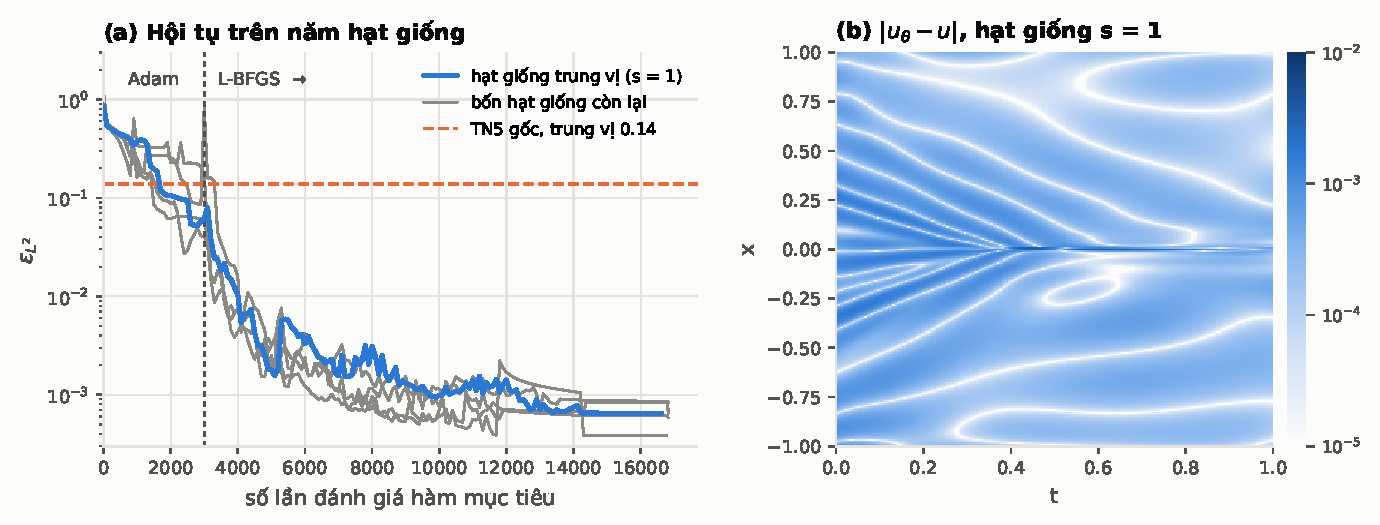
\includegraphics[width=\textwidth]{Images/chap_5/fig57_tn10.pdf}
\caption[Hội tụ của TN10 trên năm hạt giống]{Thí nghiệm~\ref{tn:tangcuong}.
(a) Sai số $\varepsilon_{L^2}$ theo số lần đánh giá hàm mục tiêu, cả năm hạt
giống; đường xanh là hạt giống \emph{trung vị}, không phải hạt giống tốt nhất.
Đường cam là trung vị của TN5. (b) Sai số tuyệt đối $\abs{u_{\btheta} - u}$ của
hạt giống trung vị, thang logarit, tính lại ở độ chính xác kép từ trọng số đã
lưu.}
\label{fig:tn10}
\end{figure}

\textbf{Kết quả 1: lời giải thích ``do ngân sách'' đứng vững, và với biên độ
lớn.} Trung vị giảm từ $1{,}38\times10^{-1}$ xuống $6{,}48\times10^{-4}$ ---
\emph{hai trăm mười ba lần}. Hạt giống \emph{tệ nhất} của TN10
($8{,}33\times10^{-4}$) vẫn tốt hơn hạt giống \emph{tốt nhất} của TN5
($7{,}93\times10^{-3}$) gần mười lần; hai khoảng cách nhau hơn một bậc độ lớn.
Kết quả nằm cùng bậc với $6{,}7\times10^{-4}$ mà công trình gốc~\cite{raissi2019}
báo cáo cho cùng kiến trúc --- tuy đó là một lần chạy, đo so với một nghiệm tham
chiếu khác, nên ta chỉ khẳng định \emph{cùng bậc} chứ không so từng chữ số. Tiêu
chí đặt trước ($< 10^{-2}$) đạt với dư hơn một bậc.

\textbf{Kết quả 2: độ phân tán giữa các hạt giống co lại.} Hệ số max/min giảm từ
$26{,}4$ ở TN5 xuống $2{,}2$ --- ngang mức của bài toán khuếch tán
(Bảng~\ref{tab:tn8-eps}). Điều Mục~\ref{sec:tn8} ghi nhận là ``trên Burgers,
ngưỡng đọc số phải là một bậc độ lớn'' hoá ra là đặc điểm của \emph{chế độ huấn
luyện chưa hội tụ}, không phải của bài toán: khi tối ưu hoá đi đủ xa, các hạt
giống hội tụ về cùng một mức.

\textbf{Kết quả 3: sai số lớn nhất vẫn ở lớp sốc, nhưng phần lớn sai số $L^2$
thì không còn ở đó.} Tỉ số $\varepsilon_{L^\infty}/\varepsilon_{L^2}$ gần như
không đổi --- khoảng $15$ ở Mục~\ref{sec:tn5}, khoảng $13$ ở TN10 --- và điểm
sai số lớn nhất của hạt giống trung vị,
$\abs{u_{\btheta} - u} = 5{,}64\times10^{-3}$, nằm tại $x \approx 0{,}002$,
$t = 0{,}45$: ngay trong lớp sốc. Nhưng một phép đếm trực tiếp trên lưới đánh giá
cho bức tranh khác với cách đọc ở Mục~\ref{sec:tn5}. Dải $\abs{x} < 0{,}02$ sau
thời điểm hình thành sốc $t_b = 1/\pi$ chiếm $1{,}4\%$ diện tích miền nhưng chỉ
chứa $12{,}4\%$ tổng bình phương sai số; ngoài dải ấy, sai số lớn nhất là
$1{,}64\times10^{-3}$ và trung vị là $2{,}2\times10^{-4}$. Nói cách khác, lớp sốc
vẫn là nơi sai số \emph{đậm đặc} nhất --- gấp khoảng chín lần mức trung bình
theo diện tích --- nhưng gần $90\%$ của $\varepsilon_{L^2}$ nay đến từ vùng
\emph{trơn}, nơi sai số trải đều ở mức $10^{-4}$ (Hình~\ref{fig:tn10}(b)).

Hệ quả thực hành: muốn hạ $\varepsilon_{L^2}$ thêm nữa, việc cần làm không còn
chủ yếu là xử lý lớp sốc. Mức nền $10^{-4}$ trên vùng trơn là giới hạn của tối
ưu hoá hoặc của khả năng xấp xỉ trên \emph{toàn} miền --- một chế độ khác với
chế độ mà Bảng~\ref{tab:ba-nguyen-nhan} mô tả cho TN5.

\begin{nhanxet}[Không được quy công cho RAR]
\label{nx:khong-quy-cong-rar}
TN10 đổi \emph{bốn} thứ cùng lúc, nên không thể tách đóng góp của từng thứ. Số
liệu theo giai đoạn ở Bảng~\ref{tab:tn10-ketqua} còn chỉ ra một điều cụ thể hơn:
\emph{phần lớn} cải thiện đến \emph{trước} khi có bất kỳ điểm RAR nào. Sau đợt
L-BFGS thứ nhất --- mạng sâu hơn, $N_r = 10\,000$, chưa một điểm thích nghi ---
trung vị đã tốt hơn TN5 $87$ lần; tính theo thang logarit, đó là khoảng $83\%$
của toàn bộ mức cải thiện $213$ lần. Năm đợt còn lại chỉ thêm hệ số $2{,}4$, và
hệ số ấy \emph{cũng} không quy được cho RAR, vì năm đợt ấy đồng thời là năm đợt
L-BFGS nữa.

Quá trình cũng không đơn điệu: hạt giống $0$ tăng sai số ở đợt thứ ba
($9{,}83\times10^{-4} \to 1{,}08\times10^{-3}$) và hạt giống $1$ ở đợt thứ tư
($9{,}80\times10^{-4} \to 1{,}51\times10^{-3}$), trước khi giảm lại. Điều này
không mâu thuẫn gì: L-BFGS cực tiểu hoá $J$, không cực tiểu hoá
$\varepsilon_{L^2}$, và mỗi lần thêm điểm RAR là thay đổi chính hàm $J$.

Vì vậy, hạn chế~(4) ở Mục~\ref{sec:hanche} chỉ được giải quyết một nửa: RAR đã
được \emph{dùng}, nhưng vai trò riêng của nó vẫn chưa được \emph{đo}. Muốn đo
cần một thí nghiệm tách biến --- cùng cấu hình TN10, bỏ RAR, cùng số đợt L-BFGS
--- trên năm hạt giống.
\end{nhanxet}

\textbf{Kết quả 4: chi phí --- khoảng cách với sai phân hữu hạn vẫn bốn bậc.}
Mục~\ref{sec:tn9} đo được PINN chậm hơn sai phân hữu hạn $1{,}8\times10^{4}$
lần ở mức sai số của TN5. Câu hỏi tự nhiên là khoảng cách ấy có thu hẹp khi đòi
hỏi độ chính xác cao hơn hay không. Ta lặp đúng quy trình của Mục~\ref{sec:tn9}:
với mỗi $N_x \in \{63, 127, 255, 511, 1\,023\}$ chọn bước thời gian \emph{lớn
nhất} vẫn nhỏ hơn một nửa chặn ổn định của chính lưới ấy, và dừng ở lưới thô
nhất đạt sai số $\le 6{,}48\times10^{-4}$.

\begin{table}[H]
\centering
\caption[Chi phí TN10 so với sai phân hữu hạn]{Chi phí để đạt mức sai số của
TN10. Thời gian sai phân là trung vị ba lần chạy.}
\label{tab:tn10-chiphi}
\small
\begin{tabular}{@{}l r r r@{}}
\toprule
\textbf{Phương pháp} & $\Delta t$ & \textbf{Thời gian} & $\varepsilon_{L^2}$ \\
\midrule
PINN, TN10, hạt giống trung vị, chạy riêng một lõi
  & --- & $38{,}7$ phút & $6{,}48\times10^{-4}$ \\
\addlinespace
Sai phân, $N_x = 511$ & $1\times10^{-3}$ & $0{,}044$ s & $2{,}65\times10^{-3}$ \\
Sai phân, $N_x = 1\,023$ & $2{,}5\times10^{-4}$ & $0{,}21$ s
  & $6{,}14\times10^{-4}$ \\
\midrule
\multicolumn{4}{@{}l@{}}{\emph{PINN chậm hơn khoảng $1{,}1\times10^{4}$ lần ở cùng mức
sai số.}} \\
\bottomrule
\end{tabular}
\end{table}

Tỉ số giảm từ $1{,}8\times10^{4}$ ở Mục~\ref{sec:tn9} xuống $1{,}1\times10^{4}$
--- thu hẹp khoảng $1{,}6$ lần, nhưng vẫn \emph{bốn} bậc độ lớn. Lý do đọc được
ngay từ hai bảng: để giảm sai số từ mức TN5 xuống mức TN10, PINN tốn thêm khoảng
$14$ lần thời gian ($170$ s $\to$ $38{,}7$ phút), còn sai phân hữu hạn tốn thêm
khoảng $21$ lần ($0{,}0098$ s $\to$ $0{,}21$ s). Hai phương pháp trả giá cho độ
chính xác theo những tỉ lệ \emph{gần nhau}, nên khoảng cách về bậc giữ nguyên;
muốn tỉ số đổi bậc thì chi phí của sai phân phải tăng nhanh hơn hẳn chi phí của
PINN, điều mà ở $d = 1$ không xảy ra.

Hai lưu ý để con số được đọc đúng. \emph{Thứ nhất}, năm hạt giống được chạy song
song trên bốn lõi, nên thời gian $51$ phút ghi trong nhật ký bị kéo dài bởi
tranh chấp CPU; con số trong bảng lấy từ một lần chạy lại hạt giống trung vị
\emph{một mình}. Lần chạy lại ấy cho lại kết quả giống \emph{từng bit} ---
$\varepsilon_{L^2}$, $\varepsilon_{L^\infty}$, số lần đánh giá, và cả $168$ điểm
trên đường sai số --- một kiểm chứng trực tiếp cho quy ước tái lập ở
Mục~\ref{sec:hanche}, hạn chế~(7).
\emph{Thứ hai}, sai số của lưới sai phân được đo so với nghiệm tham chiếu của
\emph{cùng} lược đồ trên lưới mịn hơn, nên sai số rời rạc hoá của hai lưới có
tương quan và phép đo có thể hơi lạc quan cho sai phân. Nhưng ngay cả khi phải
lên tới chính lưới tham chiếu $N_x = 2\,047$ --- chạy trong $2{,}1$ giây ---
tỉ số vẫn ở bậc $10^{3}$.

Kết luận của Nhận xét~\ref{nx:doc-tn9} vì vậy được củng cố chứ không bị lung
lay: TN10 chứng minh rằng PINN \emph{có thể} đạt độ chính xác cao trên bài toán
cứng này, nhưng không làm nó rẻ hơn. Giá trị của phương pháp vẫn phải được biện
minh ở ba động lực của Mục~\ref{subsec:gioi-han-co-dien}.

%==============================================================================
\section{Đối chiếu lý thuyết và thực nghiệm}
\label{sec:doi-chieu}
%==============================================================================
 
\begingroup
\small
\setlength{\LTcapwidth}{\textwidth}
\begin{longtable}{@{}p{2.9cm}p{3.7cm}p{3.9cm}p{3.0cm}@{}}
\caption{Đối chiếu giữa các kết quả lý thuyết và số liệu đo được.}
\label{tab:doi-chieu} \\
\toprule
\textbf{Kết quả} & \textbf{Dự báo} & \textbf{Đo được} & \textbf{Kết luận} \\
\midrule
\endfirsthead
\multicolumn{4}{@{}l}{\emph{Bảng~\thetable{} (tiếp theo)}} \\
\toprule
\textbf{Kết quả} & \textbf{Dự báo} & \textbf{Đo được} & \textbf{Kết luận} \\
\midrule
\endhead
\midrule
\multicolumn{4}{r@{}}{\emph{(xem tiếp trang sau)}} \\
\endfoot
\bottomrule
\endlastfoot
Hệ quả~\ref{hq:pinn-hong}
& $\nabla_{\btheta}J_r \equiv \bm{0}$ với ReLU
& $\norm{\nabla J_r}_\infty = 0{,}0$; $J_r = 776{,}23$ so với $778{,}49$ trên
  lưới đánh giá
& \textbf{Khớp chính xác} \\[4pt]
Mệnh đề~\ref{md:phat-bien-phat}
& sai số biên $\propto \lambda_b^{-1}$
& giảm đơn điệu ở $5/5$ hạt giống, nhưng số mũ trung vị $-0{,}64$, khoảng
  $[-0{,}907;\ -0{,}503]$
& \textbf{Khớp về hướng}, số mũ nông hơn (Mục~\ref{sec:tn8}) \\[4pt]
Mục~\ref{sec:tn2}, $\lambda_b$ tối ưu
& (không có mệnh đề)
& $\lambda_b = 100$ cực tiểu hoá $\varepsilon_{L^2}$ ở $5/5$ hạt giống
& \textbf{Khớp}: tối ưu là hữu hạn \\[4pt]
Mục~\ref{subsec:adam-vs-lbfgs}
& tựa Newton vượt điều kiện số xấu và sàn nhiễu
& cải thiện $28{,}6$ lần sau $500$ vòng
& \textbf{Khớp} \\[4pt]
Định nghĩa~\ref{dn:rho}
& bệnh lý chỉ ở bài toán cứng
& $\max\rho_b$ trên năm hạt giống: $[603;\ 4\,070]$ (Burgers) so với
  $[19{,}5;\ 96{,}5]$ (khuếch tán), hai khoảng không giao nhau
& \textbf{Khớp} về độ lớn; chiều biến thiên chỉ vững ở bài toán cứng
  (Mục~\ref{sec:tn8}) \\[4pt]
Giả thuyết \eqref{eq:pho-hieu-dung}
& phần dư ưu tiên $k$ cao
& thứ tự học đảo chiều ở $5/5$ hạt giống, nhưng $\abs{c_1}/\abs{c_8}$ trung vị
  chỉ $5{,}5$, khoảng $[4{,}5;\ 46{,}3]$
& \textbf{Khớp về hướng}, không về độ lớn \\[4pt]
Nhận xét~\ref{rem:ntk-view}
& hồi quy học tần số thấp trước
& $t_{10}$ tăng đơn điệu theo $k$ ở $5/5$ hạt giống, ba khoảng tách bạch hoàn
  toàn
& \textbf{Khớp}, vững nhất chương \\[4pt]
Mục~\ref{subsec:he-qua-pinn}
& lớp sốc học chậm nhất
& với Poisson thì ngược lại
& \textbf{Cần siết lại} (Nhận xét~\ref{nx:hieu-chinh}) \\[4pt]
Quan hệ $\rho_b$--$\norm{\bW^{(1)}}^2$
& (không có mệnh đề)
& thuyết phục trên một hạt giống, nhưng tương quan log trên năm hạt giống chỉ
  còn $0{,}24$
& \textbf{Không tái lập được} (Nhận xét~\ref{nx:tuong-quan-hong}) \\[4pt]
Thuật toán~\ref{alg:annealing}
& cân bằng biên độ gradient
& làm xấu ở $10/10$ lần chạy: trung vị $19{,}6$ lần (khuếch tán), $2{,}5$ lần
  (Burgers)
& \textbf{Có chế độ hỏng} (Bổ đề~\ref{bd:phan-hoi-duong}) \\[4pt]
Mệnh đề~\ref{md:chan-on-dinh}
& $\norm{e}_{L^2}\le \pi^{-2}\norm{r}_{L^2}$ khi điều kiện biên thoả chính xác
& tỉ số $\le 0{,}026$ trên bốn bậc độ lớn của $\norm{r}$; vi phạm $96$ lần khi
  $\lambda_b = 0{,}01$
& \textbf{Khớp}, và giả thiết biên tỏ ra thiết yếu \\[4pt]
Mệnh đề~\ref{md:chan-suy-bien}
& hằng số ổn định tỉ lệ $1/\nu$
& chặn đúng $15/15$; nhưng số mũ của tỉ số quan sát được là
  $-0{,}730 / -0{,}237 / +0{,}049$ tuỳ hạt giống, và $0/3$ hạt giống hội tụ tại
  $\nu = 0{,}01$
& \textbf{Chặn khớp, cơ chế không} (Nhận xét~\ref{nx:doc-tn7}) \\[4pt]
Mệnh đề~\ref{md:chi-phi-bp}
& $\mathrm{cost}(\nabla_{\btheta}J) \le c\cdot\mathrm{cost}(J)$ với $c\le 3$
& $c$ trung vị $2{,}67$, khoảng $[2{,}21;\ 3{,}03]$ trên mười lần đo
& \textbf{Khớp} ($9/10$ lần đo dưới chặn) \\[4pt]
Nhận xét~\ref{nx:chi-phi-bac-cao}
& đồ thị tối ưu dài gấp $4$--$6$ lần đồ thị xuôi
& trung vị $8{,}4$, khoảng $[4{,}6;\ 9{,}4]$; nhiễu đo chỉ kéo tỉ số xuống nên
  ước lượng ít chệch nhất là $\approx 9$
& \textbf{Ước lượng thấp}, cần sửa (Mục~\ref{sec:tn9})
\end{longtable}
\endgroup
 
Trong mười bốn hạng mục: sáu khớp trọn vẹn, hai khớp về hướng nhưng không về độ
lớn, \emph{bốn} cần siết lại cách phát biểu, một không tái lập được trên năm hạt
giống, và một cho kết quả tiêu cực nhưng đã truy được nguyên nhân.

Mức khớp này ủng hộ khung lý thuyết của Chương~\ref{chap:pinn} một cách
\emph{có điều kiện}, và điều kiện ấy hiện ra rất rõ khi xếp mười bốn hạng mục
theo \emph{nguồn gốc} của phát biểu thay vì theo kết quả.

Trong mười bốn hạng mục, \emph{sáu} là mệnh đề đã được chứng minh trong báo cáo
và \emph{tám} thì không. Ranh giới giữa hai nhóm ấy giải thích gần như toàn bộ
bảng.

\emph{Nhóm thứ nhất --- sáu mệnh đề đã chứng minh --- không có cái nào bị số
liệu bác bỏ.} Bốn được xác nhận trọn vẹn: Hệ quả~\ref{hq:pinn-hong},
Mệnh đề~\ref{md:san-nhieu}, Mệnh đề~\ref{md:chan-on-dinh},
Mệnh đề~\ref{md:chi-phi-bp}. Hai mệnh đề còn lại ---
Mệnh đề~\ref{md:phat-bien-phat} và Mệnh đề~\ref{md:chan-suy-bien} --- đúng về
\emph{hướng} ở mọi hạt giống và mọi giá trị $\nu$; cái phải sửa ở cả hai là
\emph{cách đọc}, không phải nội dung.

\emph{Nhóm thứ hai --- tám hạng mục không phải mệnh đề --- thì phân hoá.} Hai
khớp trọn vẹn: quan sát rằng $\lambda_b$ tối ưu là hữu hạn, và
Nhận xét~\ref{rem:ntk-view} về thứ tự học của hồi quy. Một là \emph{chế độ hỏng
tìm được} của một thuật toán trong tài liệu, và chính nó sinh ra
Bổ đề~\ref{bd:phan-hoi-duong}. \emph{Năm} hạng mục còn lại phải điều chỉnh.

Cộng cả hai nhóm: \emph{bảy hạng mục} phải điều chỉnh --- hai cách đọc mệnh đề
và năm phát biểu không phải mệnh đề. Trong toàn bộ chương thực nghiệm, chứng
minh chưa một lần thất bại; chỉ có suy đoán thất bại.

Bảy hạng mục ấy mang \emph{tám} khiếm khuyết, vì giả thuyết
\eqref{eq:pho-hieu-dung} mắc cả hai kiểu cùng lúc. Tám khiếm khuyết chia thành
bốn kiểu suy luận yếu hơn.

\emph{(i) Đối chiếu một số mũ đo ở ngân sách hữu hạn với số mũ tiệm cận.} Đây là
kiểu phổ biến nhất và tinh vi nhất, vì nó luôn cho cảm giác ``khớp gần đúng'':
Mệnh đề~\ref{md:phat-bien-phat} (số mũ đo được trải $[-0{,}907;\ -0{,}503]$ so
với dự báo $-1$) và Mệnh đề~\ref{md:chan-suy-bien} (số mũ trải
$[-0{,}730;\ +0{,}049]$ so với dự báo $-1$). Trong cả hai, độ phân tán của chính
số mũ lớn hơn khoảng cách tới dự báo, nên phép đối chiếu không mang thông tin.

\emph{(ii) Ghép hai kết quả rời rạc}: giả thuyết \eqref{eq:pho-hieu-dung} nhân
$\abs{P}^2$ với $\widehat{\varkappa}$, và kết luận ở Mục~\ref{subsec:he-qua-pinn}
ngầm giả định thừa số nào thắng.

\emph{(iii) Khái quát hoá từ một lần chạy}: quan hệ $\rho_b$--$\norm{\bW^{(1)}}^2$
không sống sót qua năm hạt giống (Nhận xét~\ref{nx:tuong-quan-hong}); phát biểu
về chiều biến thiên của $\rho_b$ trên bài toán lành mạnh chỉ đúng ở $3/5$ hạt
giống; và tỉ số $\abs{c_1}/\abs{c_8} = 38{,}6$ đo cho
giả thuyết \eqref{eq:pho-hieu-dung} thuộc đuôi hiếm của một phân bố có trung vị
$5{,}5$ (Mục~\ref{sec:tn8}). Chính chỗ cuối này là khiếm khuyết thứ hai của
\eqref{eq:pho-hieu-dung}.

\emph{(iv) Ước lượng bậc độ lớn không được kiểm chứng}: Nhận xét~\ref{nx:chi-phi-bac-cao}
đoán bội số $4$--$6$ trong khi đo được khoảng $9$ (Mục~\ref{sec:tn9}).

Đáng chú ý là cả bốn kiểu đều \emph{không} bị phát hiện bởi một lần chạy. Ba
kiểu đầu cần nhiều hạt giống; kiểu thứ tư cần lặp phép đo thời gian. Không kiểu
nào đòi hỏi thêm lý thuyết.

Đây là bài học phương pháp luận của chương, và nó nhất quán với ranh giới mà
Chương~\ref{chap:fnn} đã vạch giữa lý thuyết xấp xỉ và lý thuyết tối ưu: những gì
được chứng minh thì đứng vững, những gì được suy đoán thì cần kiểm chứng trước khi
dùng --- và ``kiểm chứng'' ở đây có nghĩa cụ thể là \emph{nhiều hơn một hạt
giống}.
 
%==============================================================================
\section{Hạn chế của thiết kế thực nghiệm}
\label{sec:hanche}
%==============================================================================
 
Để các kết luận trên được đọc đúng phạm vi, cần nêu rõ những hạn chế sau.
 
\begin{enumerate}[label=(\arabic*),leftmargin=2.2em,itemsep=4pt]
\item \emph{Năm hạt giống là ít, và các số đơn lẻ trong chương vẫn đến từ một
lần chạy.} Nguyên tắc ở Nhận xét~\ref{nx:doi-xung-hoan-vi} --- với ít nhất
$2^{n_1}n_1!$ cực tiểu tương đương, một kết quả tốt từ một hạt giống may mắn
không phải bằng chứng về phương pháp --- nay đã được thực hiện cho \emph{mọi}
thí nghiệm có phụ thuộc ngẫu nhiên: TN2, TN3, TN4, TN5 trên năm hạt giống
(Mục~\ref{sec:tn8}) và TN7 trên ba (Mục~\ref{sec:tn7}). TN1 và TN6 không cần,
vì kết luận của chúng là một đẳng thức chính xác và một bất đẳng thức đúng hoặc
sai, không phải một con số cần ước lượng.

Hai hạn chế vẫn còn. \emph{Thứ nhất}, $n = 5$ chỉ đủ để nêu trung vị và khoảng,
không đủ cho một khoảng tin cậy thật sự; với đại lượng lệch mạnh như tỉ số
$\abs{c_1}/\abs{c_8}$ ở TN3 --- bốn hạt giống trong $[4{,}5;\ 7{,}6]$ và một tại
$46{,}3$ --- năm mẫu là quá ít để mô tả cái đuôi. \emph{Thứ hai}, các bảng ở
Mục~\ref{sec:tn1}--\ref{sec:tn7} vẫn in số của \emph{một} lần chạy, còn trung
vị và khoảng chỉ xuất hiện ở Mục~\ref{sec:tn8}. Cách trình bày đúng là gộp
chúng: mỗi ô số liệu nên là ``trung vị $[\min;\max]$'' ngay tại chỗ. Báo cáo
giữ cách trình bày hiện tại để mỗi mục còn đọc được độc lập, nhưng người đọc cần
mang Mục~\ref{sec:tn8} theo khi đọc mọi con số ở các mục trước.
 
\item \emph{Ngân sách huấn luyện hạn chế --- đã kiểm, cho Burgers.} TN1--TN9
chạy trên một lõi CPU với $4\,000$--$8\,000$ vòng Adam, so với bậc $10^5$ vòng
thường dùng trong các công trình gốc~\cite{raissi2019}, nên sai số Burgers của
Mục~\ref{sec:tn5} được đọc là giới hạn của \emph{ngân sách} chứ không của
phương pháp. Mục~\ref{sec:tn10} đã kiểm dự báo này và xác nhận nó: với cấu hình
của công trình gốc và L-BFGS dài hơn, trung vị giảm $213$ lần, xuống
$6{,}48\times10^{-4}$. Hạn chế còn lại là các thí nghiệm \emph{khác} --- đặc biệt
các số đo $\rho_b$ và độ phân tán ở TN5, TN8 --- vẫn được đo ở ngân sách nhỏ, và
Mục~\ref{sec:tn10} cho thấy ít nhất độ phân tán giữa hạt giống thay đổi hẳn khi
ngân sách tăng.
 
\item \emph{Mạng nhỏ.} Kiến trúc $2\,209$--$8\,513$ tham số nhỏ hơn đáng kể so với
chuẩn mực trong tài liệu. Nói riêng, lập luận NTK ở Nhận xét~\ref{rem:ntk-view}
giả thiết chế độ nhân tiếp tuyến \emph{hằng} (mạng vô hạn rộng); với mạng cỡ này
giả thiết ấy chỉ đúng gần đúng, nên Thí nghiệm~\ref{tn:pho} phải được hiểu là kiểm
chứng \emph{định tính} về thứ tự học, không phải kiểm chứng định lượng phổ NTK.
Đây cũng là lý do ta không rút kết luận số từ đối chiếu $38{,}6$ với $64$ ở
Mục~\ref{sec:tn3}.
 
\item \emph{Chưa khảo sát độ nhạy theo cách lấy mẫu.} Lấy mẫu siêu khối Latin ở
Bảng~\ref{tab:remedies} chưa được thử. Lấy mẫu thích nghi RAR đã được \emph{dùng}
ở Mục~\ref{sec:tn10}, nhưng cùng lúc với ba thay đổi khác, và
Nhận xét~\ref{nx:khong-quy-cong-rar} chỉ ra rằng phần lớn cải thiện đến trước
khi có điểm RAR nào. Vai trò riêng của RAR vì vậy vẫn chưa được đo; muốn đo cần
một thí nghiệm tách biến trên cùng cấu hình.
 
\item \emph{Nghiệm tham chiếu cho Burgers là nghiệm số.} Dù đã kiểm chứng hội tụ
lưới ($2{,}31\times10^{-4}$), đây vẫn không phải nghiệm giải tích, nên kết luận về
Burgers có thêm một tầng sai số so với bài toán khuếch tán ở
Mục~\ref{sec:tn4}. Thêm vào đó,
Nhận xét~\ref{nx:hai-nghiem-tham-chieu} đã nêu việc hai chương hiện dùng hai nghiệm
tham chiếu khác nhau.
 
\item \emph{Tập điểm phối trí không được đặc tả đủ.} Khuyết điểm này có hai
dạng khác nhau, và cả hai chỉ lộ ra khi cài đặt lại từ chính mô tả trong báo
cáo (Phụ lục~\ref{app:code}).

\emph{Dạng thứ nhất --- lấy mẫu ngẫu nhiên, chỉ ghi số lượng.} TN4 và TN5 lấy
điểm phối trí ngẫu nhiên, nhưng báo cáo chỉ ghi \emph{số lượng} điểm chứ không
ghi bộ sinh số ngẫu nhiên và thứ tự tiêu thụ nó. Hai thí nghiệm ấy tái lập
\emph{kết luận định tính} trọn vẹn --- $\rho_b$ giảm ở TN4 và tăng ở TN5, ủ
trọng số phản tác dụng ở cả hai --- nhưng các \emph{con số} lệch từ hai đến chín
lần.

\emph{Dạng thứ hai --- không ghi gì cả.} Mục~\ref{sec:tn3} nêu ``cùng mục tiêu,
cùng kiến trúc, cùng hạt giống'' nhưng \emph{không} nói tập điểm phối trí là gì.
Bản cài đặt kèm theo chọn lưới đều $256$ điểm; một lựa chọn khác hoàn toàn có
thể cho các số $t_{10}$ khác. Đây là chỗ đặc tả yếu nhất của cả chương.

Ngược lại, TN1, TN2, TN6, TN7 dùng lưới tất định và nghiệm tham chiếu sai phân
hữu hạn của TN5 cũng tất định; tất cả tái lập tới ba hoặc bốn chữ số có nghĩa.
Bài học: với một thí nghiệm ngẫu nhiên, \emph{số lượng} điểm không phải là đặc
tả đủ --- và với một thí nghiệm tất định, im lặng thì càng không.

\item \emph{Hạt giống cố định chưa đủ để tái lập từng chữ số.} Ngoài hạt giống,
kết quả còn phụ thuộc \emph{số luồng} của thư viện đại số tuyến tính. Đo trực
tiếp trên bài toán Poisson với mạng $(1,32,32,32,1)$: khởi tạo và vòng lặp đầu
tiên giống nhau tới từng bit ở mọi cấu hình luồng, nhưng đến vòng $1\,500$ thì
hàm mục tiêu đã lệch ở chữ số có nghĩa thứ tư ($0{,}0232628$ với một luồng,
$0{,}0232880$ với hai luồng, $0{,}0232605$ với bốn luồng). Nguyên nhân là số
luồng thay đổi \emph{thứ tự cộng dồn} trong phép nhân ma trận; sai khác cỡ
epsilon máy sinh ra ở đó được quỹ đạo tối ưu hoá khuếch đại dần.

Trên bài toán Burgers thì mức khuếch đại lớn hơn hẳn, và đủ lớn để đổi kết luận
số. Chạy lại cấu hình trọng số cố định của Mục~\ref{sec:tn5} với \emph{cùng} hạt
giống, \emph{cùng} mã, \emph{cùng} \texttt{float64}, chỉ khác số luồng:

\begin{center}
\small
\begin{tabular}{@{}l r r r@{}}
\toprule
& một luồng & nhiều luồng & hệ số \\
\midrule
$\varepsilon_{L^2}$ cuối & $1{,}38\times10^{-1}$ & $8{,}19\times10^{-2}$
  & $\mathbf{1{,}69}$ \\
$\max\rho_b$            & $603$                 & $2\,101$
  & $\mathbf{3{,}48}$ \\
$\norm{\bW^{(1)}}_F$ cuối & $3{,}608$           & $3{,}970$ & $1{,}10$ \\
\bottomrule
\end{tabular}
\end{center}

Hai lần chạy khởi tạo giống hệt nhau ($\rho_b$ ban đầu trùng tới chữ số thứ mười
lăm), nên toàn bộ chênh lệch sinh ra trong huấn luyện. Đây là cùng một hiện tượng
với đoạn trên, nhưng ở quy mô khác: trên bài toán cứng, riêng số luồng đã đổi sai
số cuối gần \emph{hai} lần và đổi $\max\rho_b$ gấp \emph{ba lần rưỡi} --- so được
với độ phân tán giữa các hạt giống ở Mục~\ref{sec:tn8}. Vì $\max\rho_b$ chính là
đại lượng dùng để chẩn đoán bệnh lý gradient, nó phải được đọc theo \emph{bậc độ
lớn} chứ không theo giá trị; kết luận ở Mục~\ref{sec:tn5} vẫn đứng vững đúng vì
nó dựa trên cách biệt hai bậc chứ không dựa trên con số $1\,758$.

Điều này không mâu thuẫn với việc dùng \texttt{float64} --- độ chính xác kép vẫn
cần thiết theo lập luận ở Mục~\ref{ssec:ad-pytorch} --- nhưng nó có nghĩa là
tuyên bố ``tái lập được'' chỉ chặt chẽ khi cố định \emph{cả} hạt giống,
\emph{cả} số luồng và \emph{cả} phiên bản thư viện. Mọi số liệu trong
Phụ lục~\ref{app:code} vì vậy được sinh với \texttt{OMP\_NUM\_THREADS=1}.

\item \emph{Không đo được hằng số ổn định ở chế độ $\nu$ rất nhỏ.}
Mục~\ref{sec:tn7} đã quét $\nu$ trên bài toán đối lưu--khuếch tán, nhưng phép đo
chỉ có nghĩa ở những $\nu$ mà huấn luyện đưa được phần dư xuống thấp. Tại
$\nu = 0{,}01$ không hạt giống nào làm được điều đó, nên chính chế độ mà
Mệnh đề~\ref{md:chan-suy-bien} nói tới lại là chế độ không kiểm chứng được bằng
PINN. Muốn tách riêng tầng thứ nhất cần một cách khác --- chẳng hạn dựng sai số
\emph{nhân tạo} theo hướng hàm riêng $\sin\pi x$ rồi đo trực tiếp tỉ số, thay vì
để quá trình huấn luyện quyết định hướng của sai số.

\item \emph{Mọi bài toán thực nghiệm đều nằm ngoài ba động lực của
Mục~\ref{subsec:gioi-han-co-dien}.} Mọi bài toán trong chương này đều là bài
toán \emph{thuận}, một chiều theo không gian, với dữ liệu biên và dữ liệu đầu
cho đầy đủ và không nhiễu --- tức không chạm tới bài toán ngược, không chạm tới
điều kiện biên khuyết, và không chạm tới lời nguyền số chiều. Đây chính là chế
độ mà phương pháp lưới cổ điển gần như tối ưu, và Mục~\ref{sec:tn9} đo được cái
giá của việc đó: chậm hơn khoảng $1{,}8\times10^{4}$ lần ở cùng mức sai số. Hệ quả cho cách đọc
chương này: các thí nghiệm ở đây kiểm chứng \emph{cơ chế} của PINNs --- vai trò
hàm kích hoạt, cái giá của ràng buộc mềm, thiên kiến phổ, bệnh lý gradient, các
chặn ổn định --- chứ không kiểm chứng \emph{tính cạnh tranh} của phương pháp.
Muốn kiểm chứng điều sau cần ít nhất một bài toán nhiều chiều hoặc một bài toán
ngược, là hướng nêu ở Chương~\ref{chap:ketluan}.
\end{enumerate}
 
%==============================================================================
\section*{Kết luận chương}
\addcontentsline{toc}{section}{Kết luận chương}
%==============================================================================
 
Chương này đã hiện thực hoá khung lý thuyết của Chương~\ref{chap:pinn} trên
PyTorch và đưa ra số liệu kiểm chứng cho từng phát biểu chính.
 
Về mặt \emph{kỹ thuật}, cơ chế đồ thị động cùng cờ \texttt{create\_graph=True} đủ
để hiện thực trực tiếp các truy hồi \eqref{eq:G-truy-hoi} và
\eqref{eq:S-truy-hoi} mà không cần lập trình tường minh $\sigma''$, đúng như
Mệnh đề~\ref{md:ad-tai-tao} bảo đảm; độ chính xác kép là điều kiện cần để phân
biệt sai số xấp xỉ với sai số làm tròn.
 
Về mặt \emph{kiểm chứng}, ba kết quả nổi bật. Thứ nhất,
Hệ quả~\ref{hq:pinn-hong} được xác nhận tới từng chữ số máy: mạng ReLU cho
gradient bằng đúng không, chứng tỏ điều kiện $\sigma \in C^m$ là bắt buộc chứ
không phải khuyến nghị. Thứ hai, bệnh lý gradient được chứng minh là hiện tượng
\emph{phụ thuộc bài toán}: trên năm hạt giống, $\max\rho_b$ của Burgers nằm trong
$[603;\ 4\,070]$ còn của khuếch tán trong $[19{,}5;\ 96{,}5]$ -- hai khoảng
không giao nhau, nên việc chẩn đoán trước khi can thiệp là bắt buộc. Ngược lại,
phát biểu về \emph{chiều} biến thiên chỉ vững ở bài toán cứng. Thứ ba, giả thuyết \eqref{eq:pho-hieu-dung} được xác nhận theo
cách bất ngờ nhất: toán tử vi phân \emph{đảo ngược} thiên kiến phổ, khiến sai số
dồn về mode tần số thấp; phát hiện này buộc phải siết lại cách phát biểu ở
Mục~\ref{subsec:he-qua-pinn}.
 
Về mặt \emph{phương pháp}, hai kết quả tiêu cực có giá trị riêng. Việc tăng
$\lambda_b$ vô hạn không phải chiến lược tốt, vì sai số $L^2$ toàn cục đạt cực
tiểu tại một giá trị hữu hạn -- điều mà Mệnh đề~\ref{md:phat-bien-phat}, vốn chỉ
theo dõi sai số biên, không thể tiên đoán. Và thuật toán ủ trọng số ở dạng nguyên
bản làm giảm độ chính xác trên cả hai bài toán; ở đây thực nghiệm không chỉ phát
hiện vấn đề mà còn dẫn tới một kết quả lý thuyết mới:
Bổ đề~\ref{bd:phan-hoi-duong} chứng minh rằng quy tắc \eqref{eq:lambda-hat} có một
chế độ phản hồi dương với tốc độ phân kỳ $\hat\lambda_i \sim J_i^{-1/2}$ và không
có cơ chế tự hãm.
 
Về mặt \emph{thực hành}, hai phép đo cuối chương trả lời hai câu hỏi mà các mục
trước để ngỏ, và cả hai câu trả lời đều khiêm tốn hơn kỳ vọng. Mục~\ref{sec:tn8}
lặp TN4 và TN5 trên năm hạt giống và cho thấy độ phân tán tự nó phụ thuộc bài
toán: hệ số $2{,}4$ giữa lần chạy tốt nhất và tệ nhất trên bài toán khuếch tán,
nhưng $26{,}4$ trên Burgers --- đủ để loại bỏ một tương quan mà chương này từng
ghi nhận (Nhận xét~\ref{nx:tuong-quan-hong}). Mục~\ref{sec:tn9} đo chi phí và
cho con số bất lợi nhất của báo cáo: PINN chậm hơn sai phân hữu hạn khoảng bốn
bậc độ lớn ở cùng mức sai số, trên đúng lớp bài toán mà cả ba động lực của
Mục~\ref{subsec:gioi-han-co-dien} đều vắng mặt.

Mục~\ref{sec:tn10} khép lại chương bằng cách làm đúng điều mà các mục trước chỉ
dự báo: áp dụng cấu hình của công trình gốc cùng lấy mẫu thích nghi cho bài toán
Burgers. Sai số trung vị giảm $213$ lần, xuống $6{,}48\times10^{-4}$ --- cùng bậc
với công trình gốc --- và độ phân tán giữa hạt giống co từ $26{,}4$ về $2{,}2$.
Nhưng kết quả tích cực nhất chương này cũng được đọc với cùng sự dè dặt như các
kết quả tiêu cực: nó không quy được cho riêng RAR
(Nhận xét~\ref{nx:khong-quy-cong-rar}), và nó chỉ thu hẹp khoảng cách chi phí
$1{,}6$ lần --- vẫn bốn bậc độ lớn.

Hai kết quả cuối cùng ấy minh hoạ đúng vai trò của chương: bước kiểm chứng số không
chỉ xác nhận hay bác bỏ lý thuyết đã có, mà còn chỉ ra chỗ lý thuyết cần được bổ
sung -- và chỉ ra cả chỗ mà chính chương thực nghiệm đã kết luận vội.
 
